\documentclass[%
	pdftex,
	a4paper,
	oneside,
	idxtotoc,
	parskip,%        European type with space paragraphs
	11pt,
	listsleft
]{scrbook}

\usepackage[utf8]{inputenc}
\usepackage[T1]{fontenc}

\usepackage{german, ngerman}
\usepackage[german]{babel}

\usepackage{a4wide}
\usepackage[left=3.0cm, right=2.5cm, top=3.0cm, bottom=3.5cm]{geometry}
\usepackage{float}

%
% Package and configuration for abbreviations and markup
%
\usepackage{nomencl}
  \let\abbrev\nomenclature
  \renewcommand{\nomname}{Abkürzungsverzeichnis}
  \setlength{\nomlabelwidth}{.25\hsize}
  \renewcommand{\nomlabel}[1]{#1 \dotfill}
  \setlength{\nomitemsep}{-\parsep}
  \makenomenclature
  
\usepackage[normalem]{ulem}
  \newcommand{\markup}[1]{\uline{#1}}

%
% Embedding graphic
%
\usepackage{graphicx}
\usepackage{path,epsfig}

\usepackage{url}

\usepackage{titlesec, blindtext, color}

\definecolor{light_gray}{gray}{0.85}
\definecolor{gray}{gray}{0.75}
\definecolor{dark_gray}{gray}{0.50}

% Chapter format
\newcommand{\hsp}{\hspace{20pt}}
\titleformat{\chapter}[hang]{\Huge\bfseries}{\thechapter\hsp\textcolor{gray}{|}\hsp}{0pt}{\Huge\bfseries}

% listings
\usepackage{listings}
\usepackage{inconsolata} 
\usepackage{blindtext,expdlist} 

\lstset{
  backgroundcolor=\color{light_gray},
  rulesepcolor=\color{gray},
  numbers=left,
  stepnumber=1,
  numberstyle=\footnotesize,
  captionpos=b,
  breaklines=true,
  breakatwhitespace=true,
  basicstyle=\footnotesize\ttfamily
}

\usepackage{fancyhdr}
\pagestyle{fancy}

%
% Package extending table properties
%
\usepackage{array}

% 
% Nicer tables
%
\usepackage{booktabs}


%
% Allow color in tables, longtables and add supertabular
%
\usepackage{colortbl}
\usepackage{tabularx}
\usepackage{longtable}
\usepackage{multirow}
\usepackage{hhline}

\usepackage{color}
\usepackage{xcolor}

\usepackage{calc}

\usepackage{ifthen} 

\sloppy
\raggedbottom

%
% Table number format: chapter + table number
%
\usepackage{chngcntr}
\counterwithin{figure}{section}
\counterwithin{table}{section}


\begin{document}
% No indentation
\parindent 0pt
\parskip 11pt

%
%
% Titelseite
%
%

\begin{titlepage}
    \begin{center}
        
\includegraphics[width=0.65\textwidth]{images/opennms-logo.png}
    \end{center}
    \vspace{8em}
    \center
    \Huge{\textbf{The Definitive Guide}}
    \vspace{15em}

    \begin{flushright}
        
\includegraphics[width=0.12\textwidth]{images/by-sa.png}
        \\
        \tiny{Ronny Trommer}
    \end{flushright}
\end{titlepage}

\tableofcontents
\addcontentsline{toc}{section}{Inhaltsverzeichnis} 
\newpage

\printnomenclature
\addcontentsline{toc}{chapter}{Abkürzungsverzeichnis}
\newpage

\listoffigures
\addcontentsline{toc}{chapter}{Abbildungsverzeichnis}
\newpage

\listoftables
\addcontentsline{toc}{chapter}{Tabellenverzeichnis}
\newpage

%=======================================================
\chapter{Konzepte des Netzwerk-Monitorings}
%=======================================================
\include{content/concepts-monitoring/introduction}
%=======================================================
\section{Einstieg in FCAPS}
%=======================================================

%=======================================================
\section{Polling vs. Events}
%=======================================================

%=======================================================
\section{Der Aufbau von OpenNMS}
%=======================================================

%=======================================================
\section{Der OpenNMS Event-Bus}
%=======================================================

\include{content/concepts-monitoring/terminology}

%=======================================================
\chapter{Netzwerk-Management Protokolle und Agenten}
%=======================================================
\include{content/nms-protocols/introduction}
\include{content/nms-protocols/snmp}
\include{content/nms-protocols/jmx}
\include{content/nms-protocols/wmi}
\include{content/nms-protocols/nrpe}
\include{content/nms-protocols/nsclient}

%=======================================================
\chapter{Planung und Design der Installation}
%=======================================================
\include{content/install/introduction}
%=======================================================
\section{Alleinstehende Installation}
%=======================================================

%=======================================================
\section{Verteilte Installation von OpenNMS}
%=======================================================

%=======================================================
\section{Konzepte für Hochverfügbarkeit}
%=======================================================

%=======================================================
\section{Best-Practices für die Installation}
%=======================================================


%=======================================================
\chapter{Anwendungs- und Service Monitoring}
%=======================================================
\include{content/service-assurance/introduction}
%=======================================================
\section{Konzepte des OpenNMS Service Monitors}
%=======================================================

\include{content/service-assurance/implementations}

%=======================================================
\chapter{Aufzeichnen von Leistungsdaten}
%=======================================================
\include{content/datacollection/introduction}
%=======================================================
\section{Konzepte der Leistungsdatenaufzeichnung}
%=======================================================

\include{content/datacollection/intro-rrd}
\include{content/datacollection/collection-snmp}
\include{content/datacollection/collection-jmx}
\include{content/datacollection/collection-wmi}
\include{content/datacollection/collection-jdbc}
\include{content/datacollection/collection-xml}
\include{content/datacollection/collection-http}
\include{content/datacollection/collection-nsclient}

%=======================================================
\chapter{Das Benachrichtigungssystem}
%=======================================================
\include{content/notification/introduction}
\include{content/notification/notify-concepts}
\include{content/notification/destination-paths}
\include{content/notification/notification-commands}
\include{content/design-notification/escalation}
\include{content/design-notification/roles-and-groups}
\include{content/notification/extending-notification-commands}

%=======================================================
\chapter{Provisioning System}
%=======================================================
\epigraphhead[70]{\epigraph{If opportunity doesn't knock, build a door.}{\textit{Milton Berle}}}
\include{content/provisioning-system/introduction}
\include{content/provisioning-system/workflow}
%=======================================================
\section{Provisioning System}
%=======================================================
Eine der grösseren Aufgaben von Netzwerk-Management-Systemen (NMS) ist es, Möglichkeiten und Wege zu bieten, wie die reale Welt in das entsprechende Modell des NMS zu überführen. Genau diese Aufgabe erfüllt bei OpenNMS das \emph{Provisioning System}. Es besteht aus einem Hintergrundprozess \emph{provisiond}.
%=======================================================
\section{Provisioning - ReST API}
%=======================================================


%=======================================================
\chapter{Inventory Integration}
%=======================================================
\epigraphhead[70]{\epigraph{The only source of knowledge is experience.}{\textit{Albert Einstein}}}
\include{content/inventory-integration/introduction}
%=======================================================
\section{DNS-Server Provisioning}
%=======================================================

%=======================================================
\section{VMware}
%=======================================================
Virtualisierung ist ein wichtiger Bestandteil heutiger IT-Landschaften geworden. In Version 1.12 wurde aus diesem Grund das \emph{Provisioning} erweitert. Es ist nun möglich direkt virtuelle Maschinen (VM) und Host-Systeme aus einer \emph{VMware} basierenden Virtualisierung in \emph{OpenNMS} zu importieren.

Typischerweise sind diese Informationen über das \emph{vCenter} zugänglich. Leistungsdaten können dort allerdings nur über einen sehr begrenzten Zeitraum gespeichert werden.

%=======================================================
\subsection{Vorbereiten VMware vCenter}
%=======================================================

\begin{figure}[H]
	\centering
	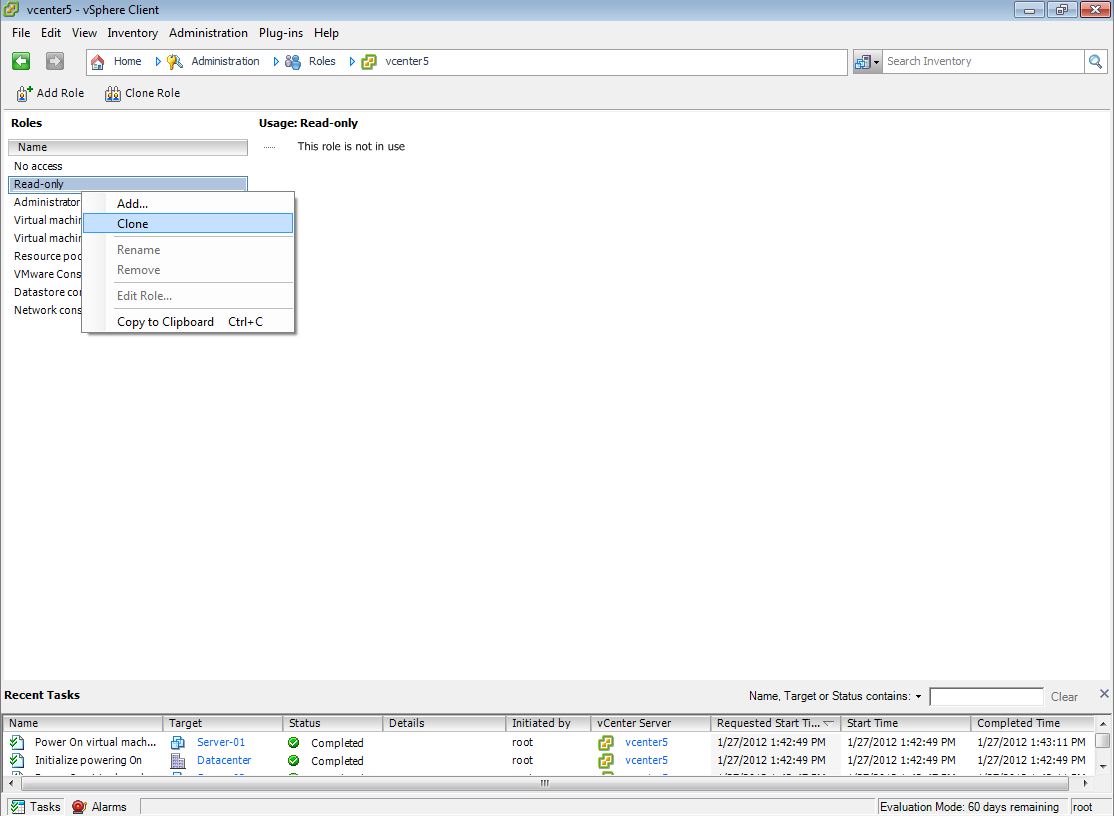
\includegraphics[width=1.0\textwidth]{images/3rd-party/vmware/0-cloning}
	\caption{Duplizieren einer \emph{Read-Only} Rolle in \emph{vCenter}}
	\label{pic:vmware-cloning}
\end{figure}

\begin{figure}[H]
	\centering
	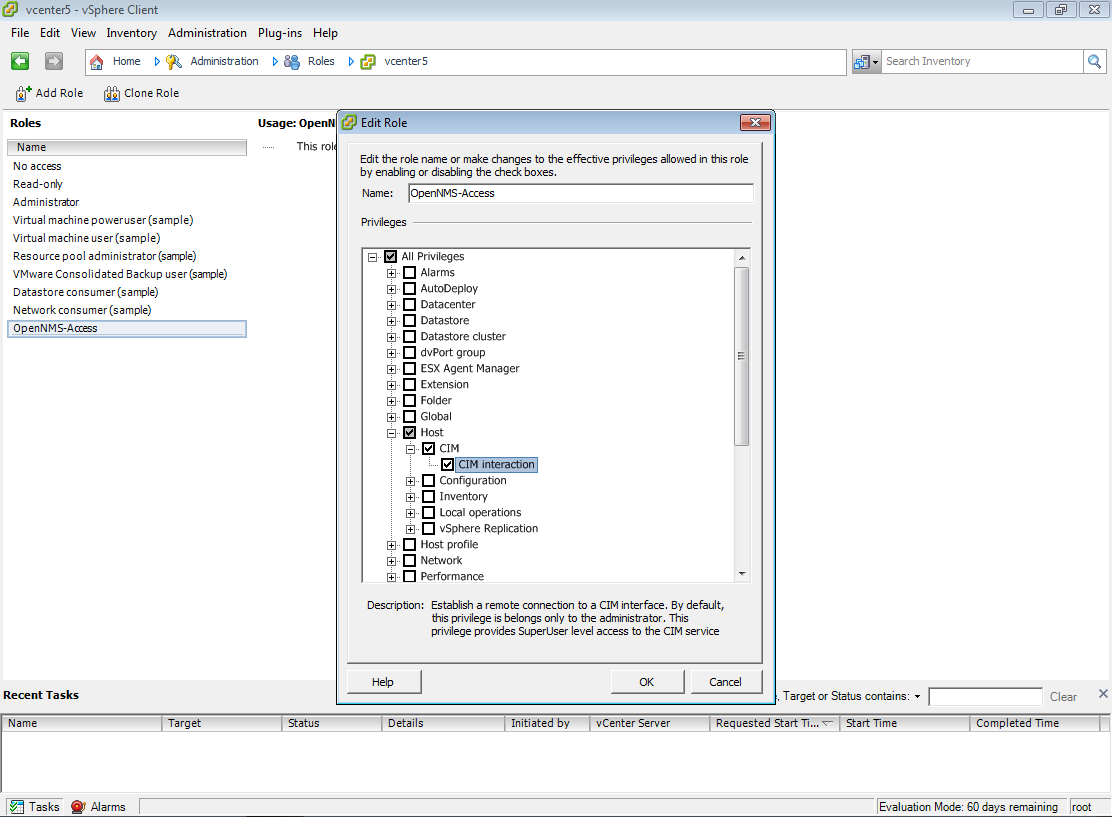
\includegraphics[width=1.0\textwidth]{images/3rd-party/vmware/1-editing}
	\caption{Duplizieren einer \emph{Read-Only} Rolle in \emph{vCenter}}
	\label{pic:vmware-editing}
\end{figure}

\begin{figure}[H]
	\centering
	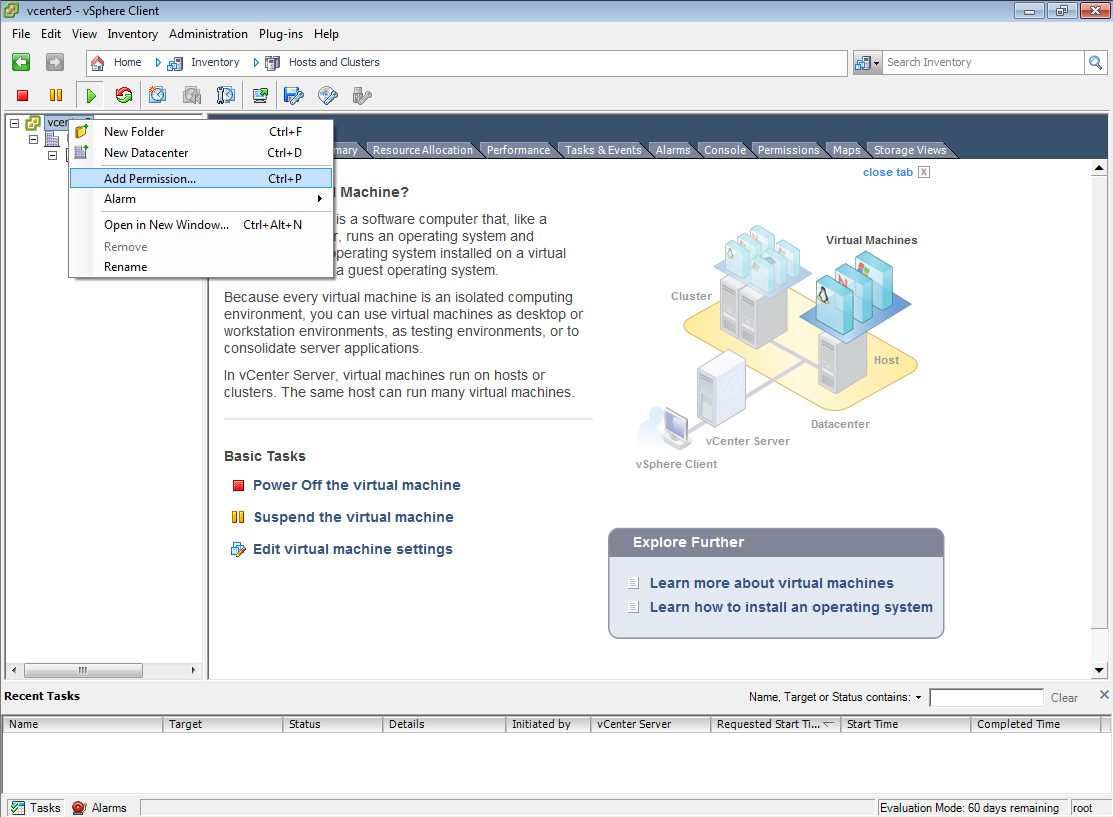
\includegraphics[width=1.0\textwidth]{images/3rd-party/vmware/2-permission}
	\caption{Duplizieren einer \emph{Read-Only} Rolle in \emph{vCenter}}
	\label{pic:vmware-permission}
\end{figure}

\begin{figure}[H]
	\centering
	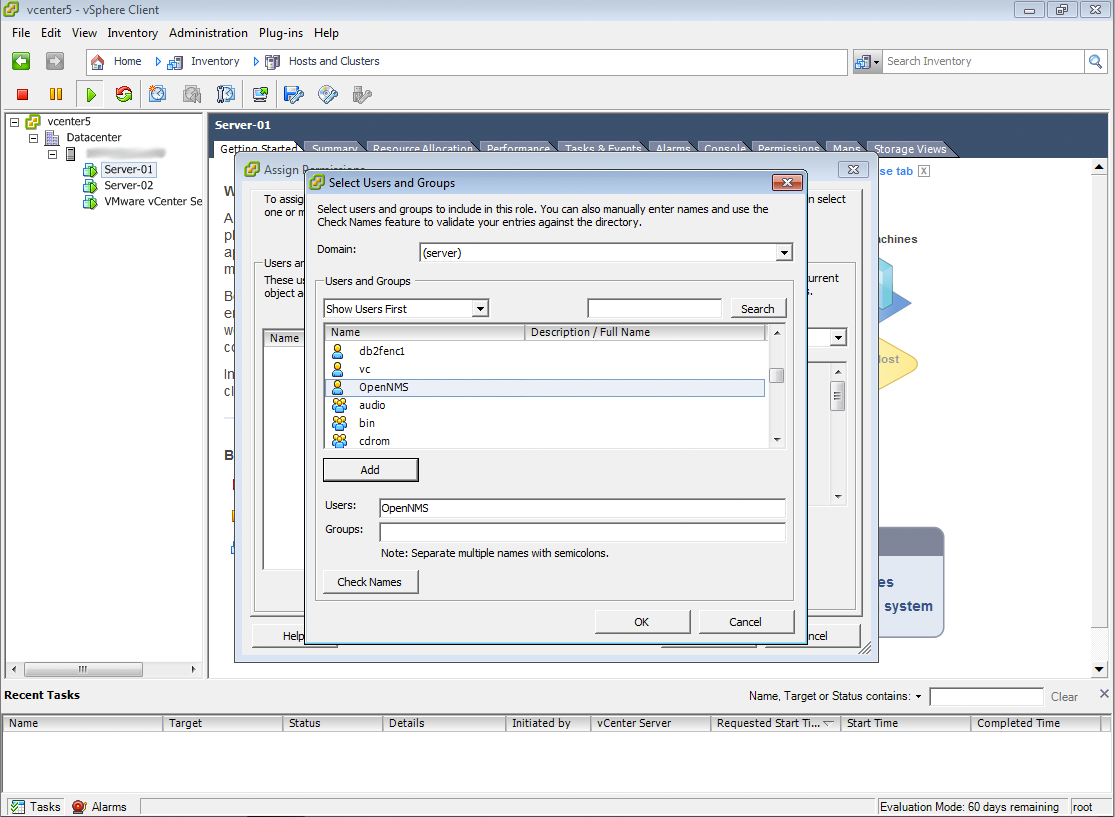
\includegraphics[width=1.0\textwidth]{images/3rd-party/vmware/3-adding}
	\caption{Duplizieren einer \emph{Read-Only} Rolle in \emph{vCenter}}
	\label{pic:vmware-adding}
\end{figure}

\begin{figure}[H]
	\centering
	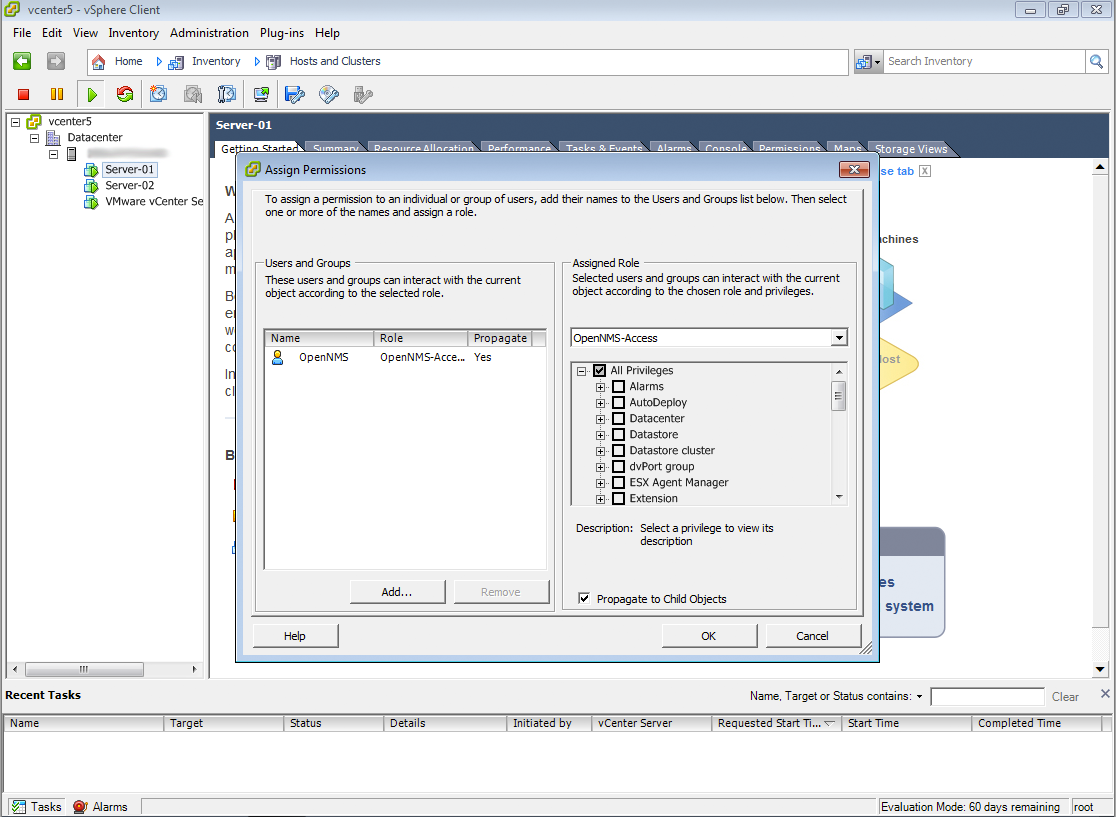
\includegraphics[width=1.0\textwidth]{images/3rd-party/vmware/4-ok}
	\caption{Duplizieren einer \emph{Read-Only} Rolle in \emph{vCenter}}
	\label{pic:vmware-ok}
\end{figure}

\begin{figure}[H]
	\centering
	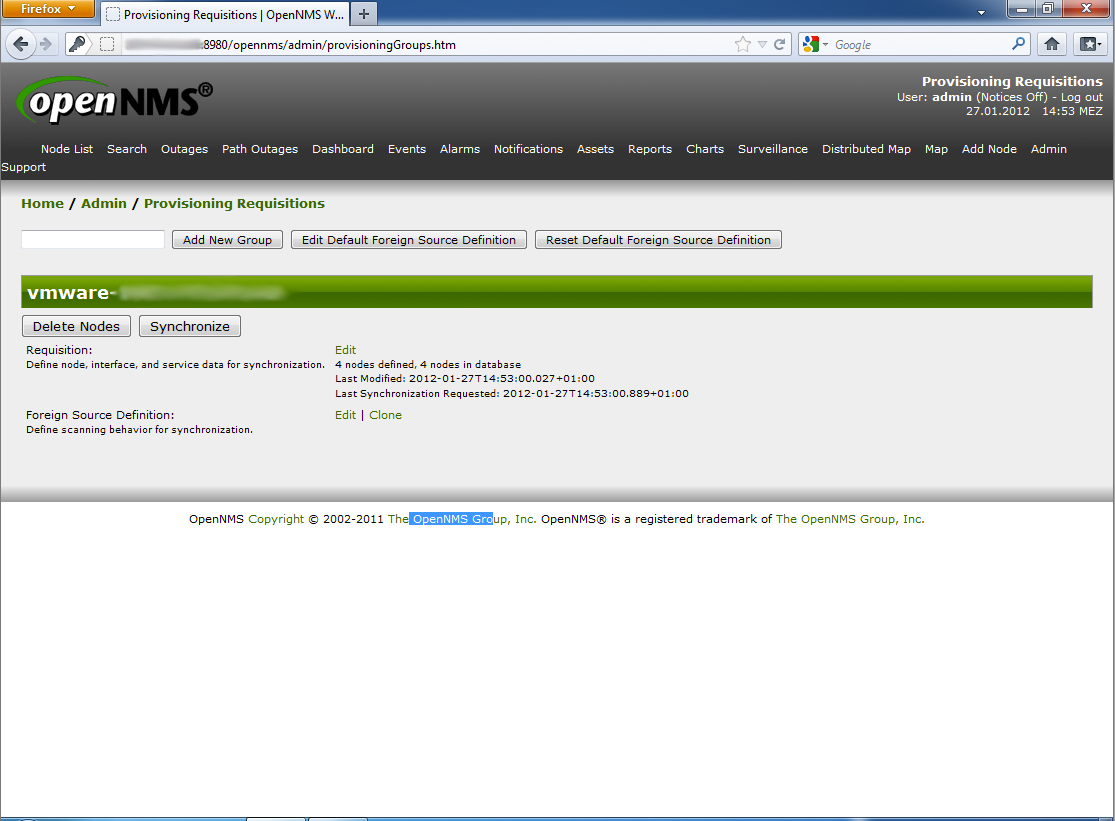
\includegraphics[width=1.0\textwidth]{images/3rd-party/vmware/5-provisioning}
	\caption{Duplizieren einer \emph{Read-Only} Rolle in \emph{vCenter}}
	\label{pic:vmware-provisioning}
\end{figure}

\begin{figure}[H]
	\centering
	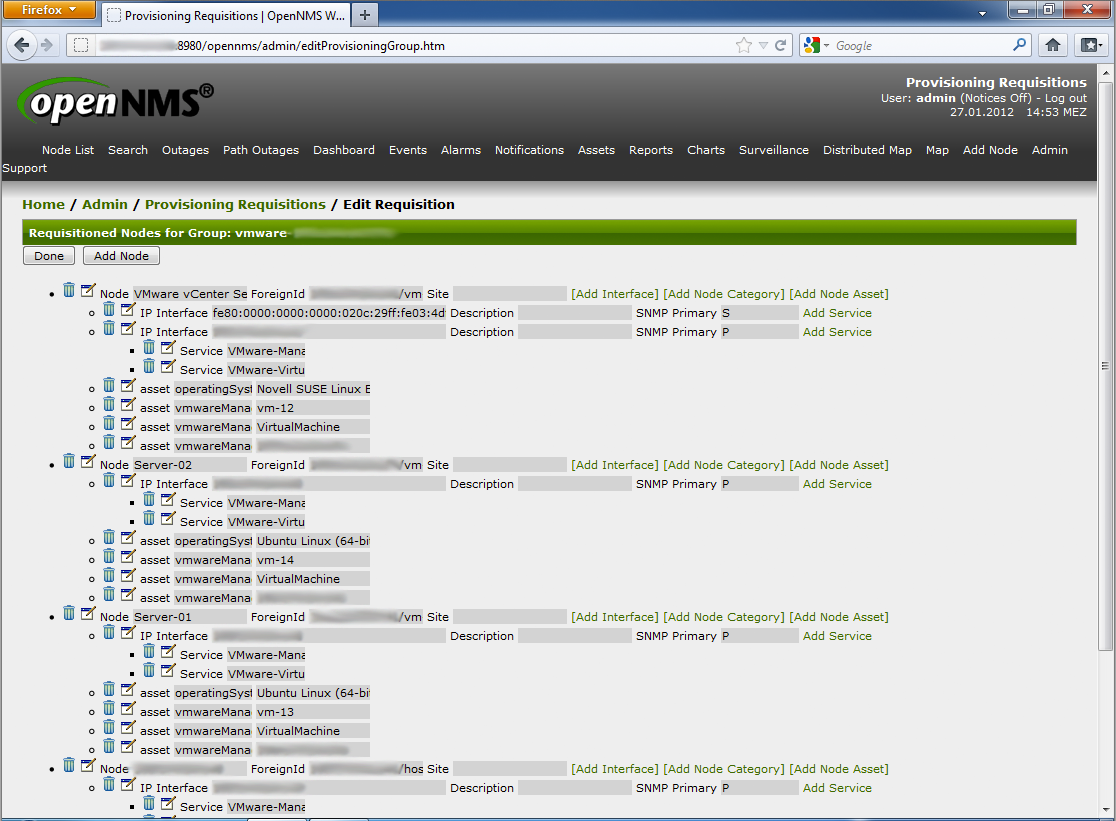
\includegraphics[width=1.0\textwidth]{images/3rd-party/vmware/6-group}
	\caption{Duplizieren einer \emph{Read-Only} Rolle in \emph{vCenter}}
	\label{pic:vmware-group}
\end{figure}

\begin{figure}[H]
	\centering
	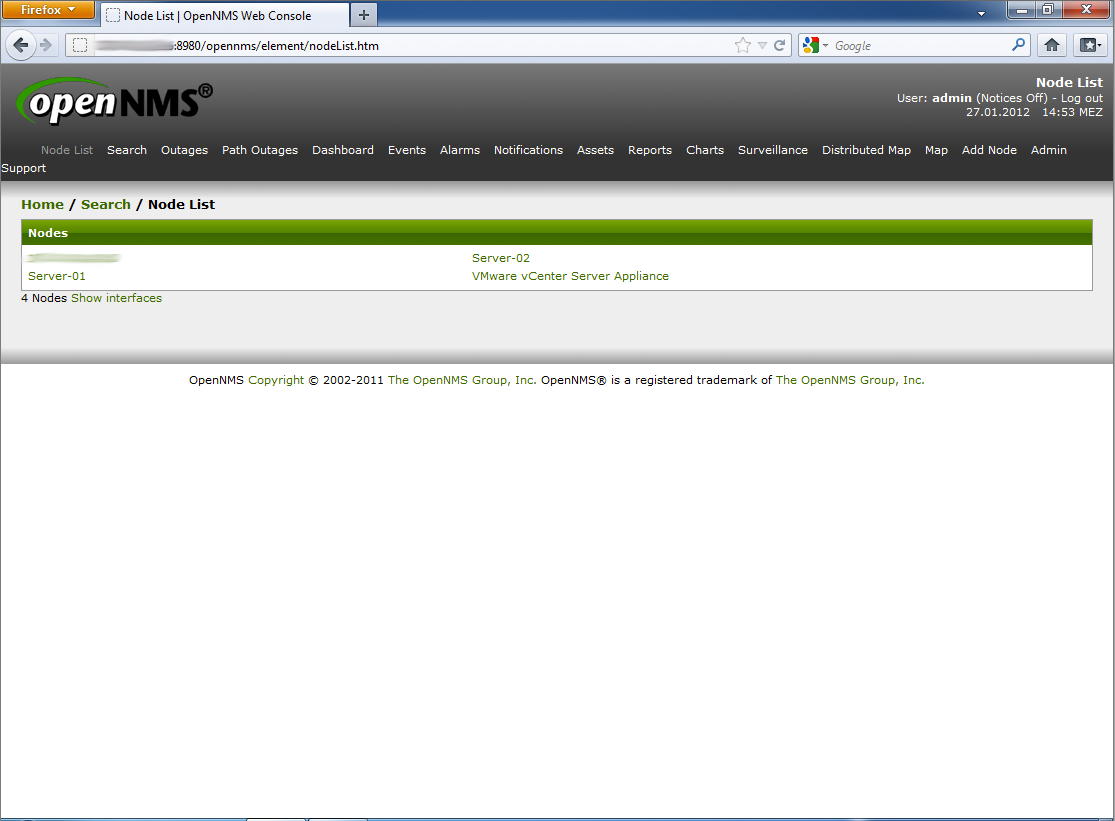
\includegraphics[width=1.0\textwidth]{images/3rd-party/vmware/7-nodes}
	\caption{Duplizieren einer \emph{Read-Only} Rolle in \emph{vCenter}}
	\label{pic:vmware-nodes}
\end{figure}

\begin{figure}[H]
	\centering
	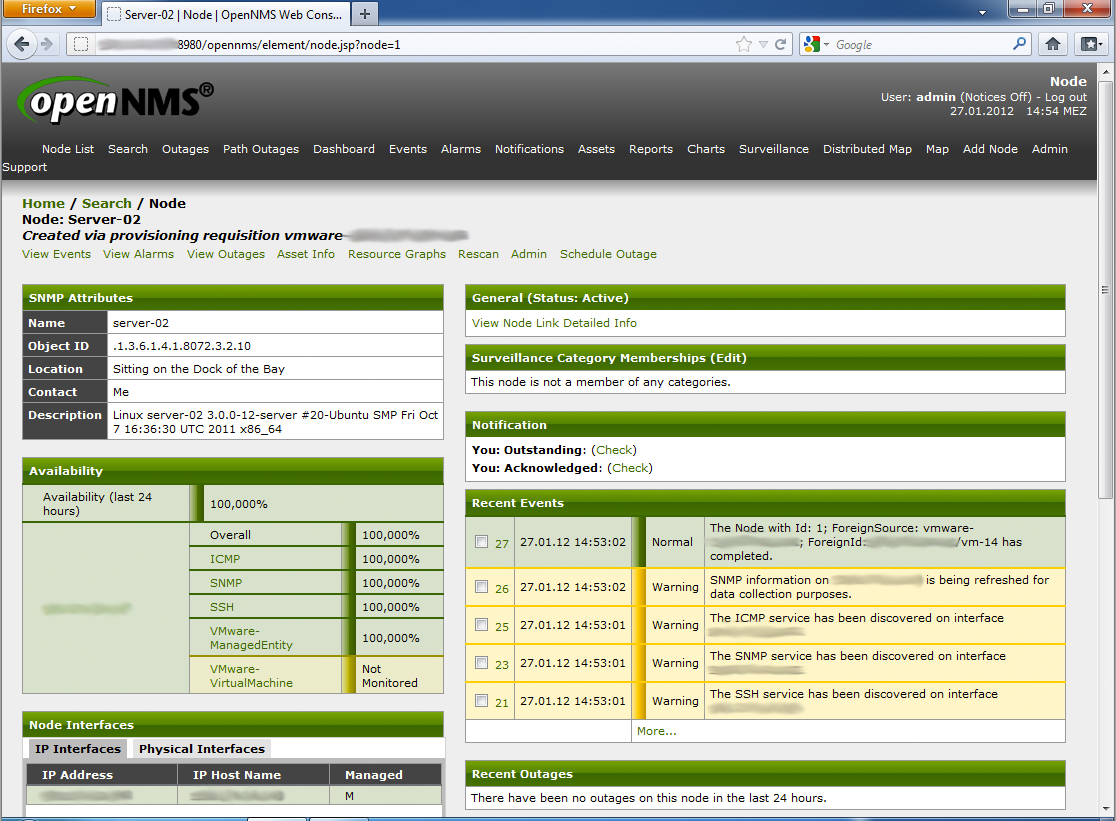
\includegraphics[width=1.0\textwidth]{images/3rd-party/vmware/8-detail}
	\caption{Duplizieren einer \emph{Read-Only} Rolle in \emph{vCenter}}
	\label{pic:vmware-detail}
\end{figure}


%=======================================================
\subsection{VMware Provisioning Adapter}
%=======================================================
In \emph{VMware vCenter} werden alle Komponenten verwaltet, die in der virtuellen Umgebung eingesetzt werden. Dort werden neben den VMs und Host-Systemen auch Leistungsdaten und der Hardwarestatus der Host-Systeme ermittelt und zur Verfügung gestellt. Um die VMs und Host-Systeme von einem bestehenden \emph{vCenter} zu importieren wurde das \emph{Provisioning} um einen \emph{Requisition-Handler} erweitert. Dieser verbindet sich zum \emph{vCenter} und liest dort alle notwendigen Informationen der VMs und Host-Systeme und überführt diese in das \emph{OpenNMS Model} für den Import.

Für den Import werden die folgenden Informationen aus vCenter ausgelesen:
\begin{itemize}
  \item \textit{}
\end{itemize}

\begin{figure}[H]
	\centering
	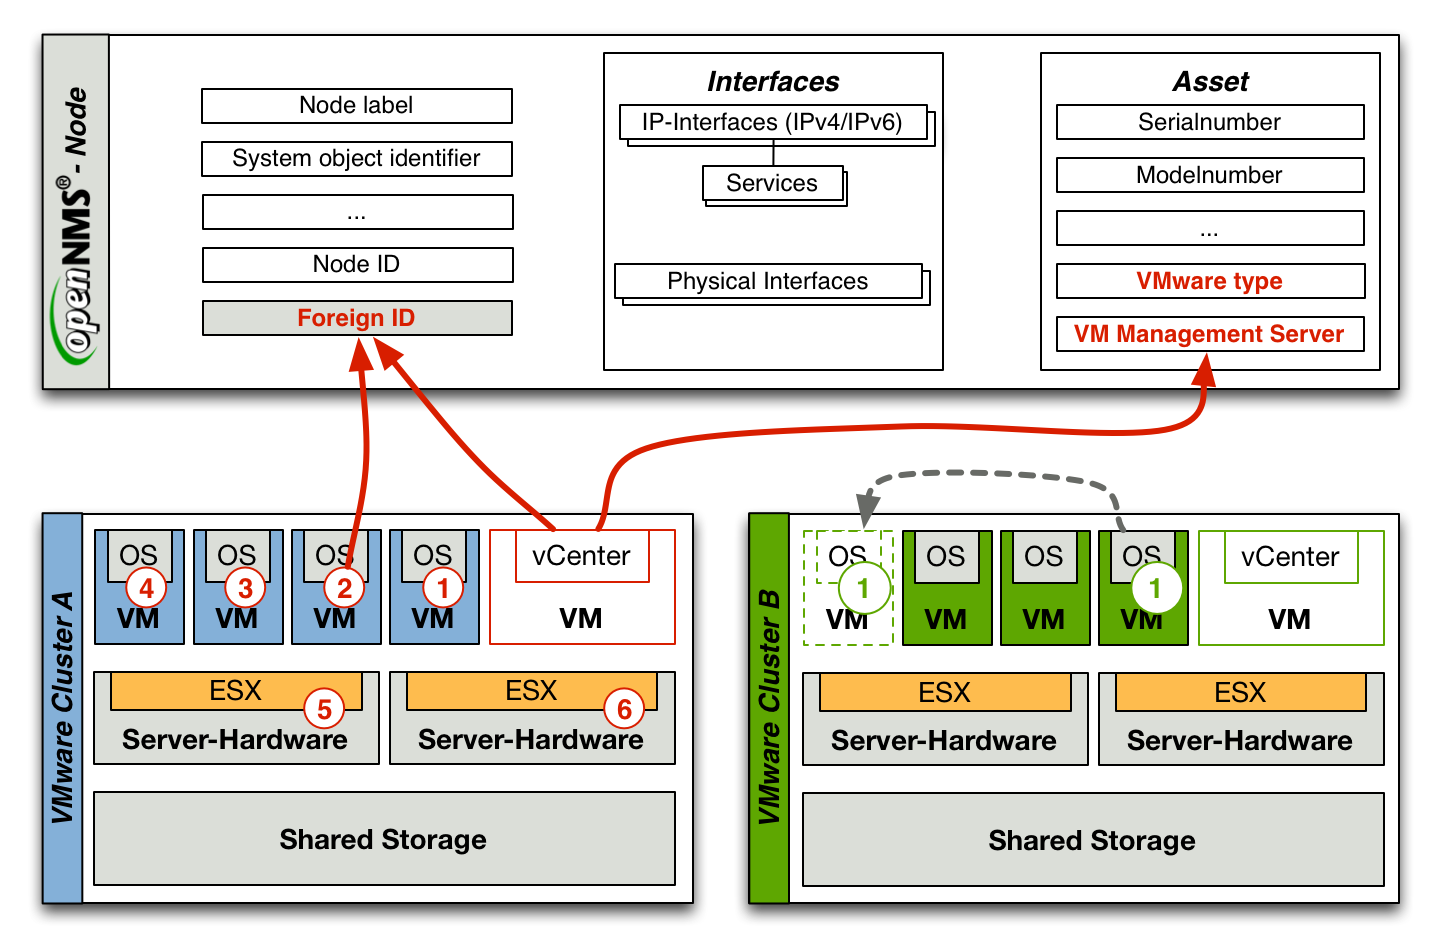
\includegraphics[width=1.0\textwidth]{images/3rd-party/vmware/vmware-cluster}
	\caption{\emph{Provisioning} mit mehreren \emph{VMware Clustern}}
	\label{pic:lab}
\end{figure}


%=======================================================
\subsection{Leistungsdaten von VMware Umgebung}
%=======================================================

%=======================================================
\subsection{Hardwarestatus von VMware Hosts}
%=======================================================

%=======================================================
\subsection{VMware und die Topology Karte}
%=======================================================
%=======================================================
\section{OCS-Inventory Provisioning}
%=======================================================


%=======================================================
\chapter{Visualisierung von Topologien}
%=======================================================
\epigraphhead[70]{\epigraph{The minute that you're not learning I believe you're dead.}{\textit{Jack Nicholson}}}
%=======================================================
\section{Karten und Topologien}
%=======================================================

%=======================================================
\subsection{Geografische Node-Karte}
%=======================================================

%=======================================================
\subsection{Topologie-Karte}
%=======================================================

%=======================================================
\subsection{Remote-Poller Karte}
%=======================================================

%=======================================================
\chapter{Inventory Integration}
%=======================================================
\epigraphhead[70]{\epigraph{The only source of knowledge is experience.}{\textit{Albert Einstein}}}
\include{content/inventory-integration/introduction}
%=======================================================
\section{DNS-Server Provisioning}
%=======================================================

%=======================================================
\section{VMware}
%=======================================================
Virtualisierung ist ein wichtiger Bestandteil heutiger IT-Landschaften geworden. In Version 1.12 wurde aus diesem Grund das \emph{Provisioning} erweitert. Es ist nun möglich direkt virtuelle Maschinen (VM) und Host-Systeme aus einer \emph{VMware} basierenden Virtualisierung in \emph{OpenNMS} zu importieren.

Typischerweise sind diese Informationen über das \emph{vCenter} zugänglich. Leistungsdaten können dort allerdings nur über einen sehr begrenzten Zeitraum gespeichert werden.

%=======================================================
\subsection{Vorbereiten VMware vCenter}
%=======================================================

\begin{figure}[H]
	\centering
	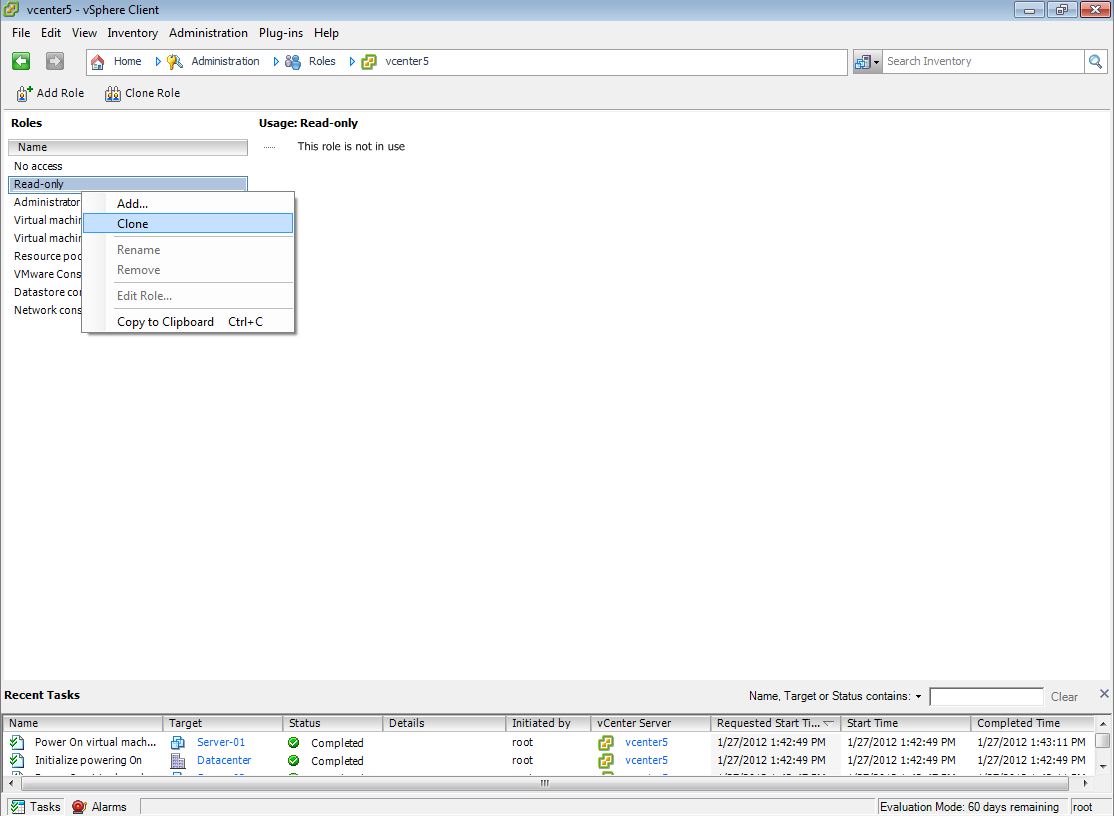
\includegraphics[width=1.0\textwidth]{images/3rd-party/vmware/0-cloning}
	\caption{Duplizieren einer \emph{Read-Only} Rolle in \emph{vCenter}}
	\label{pic:vmware-cloning}
\end{figure}

\begin{figure}[H]
	\centering
	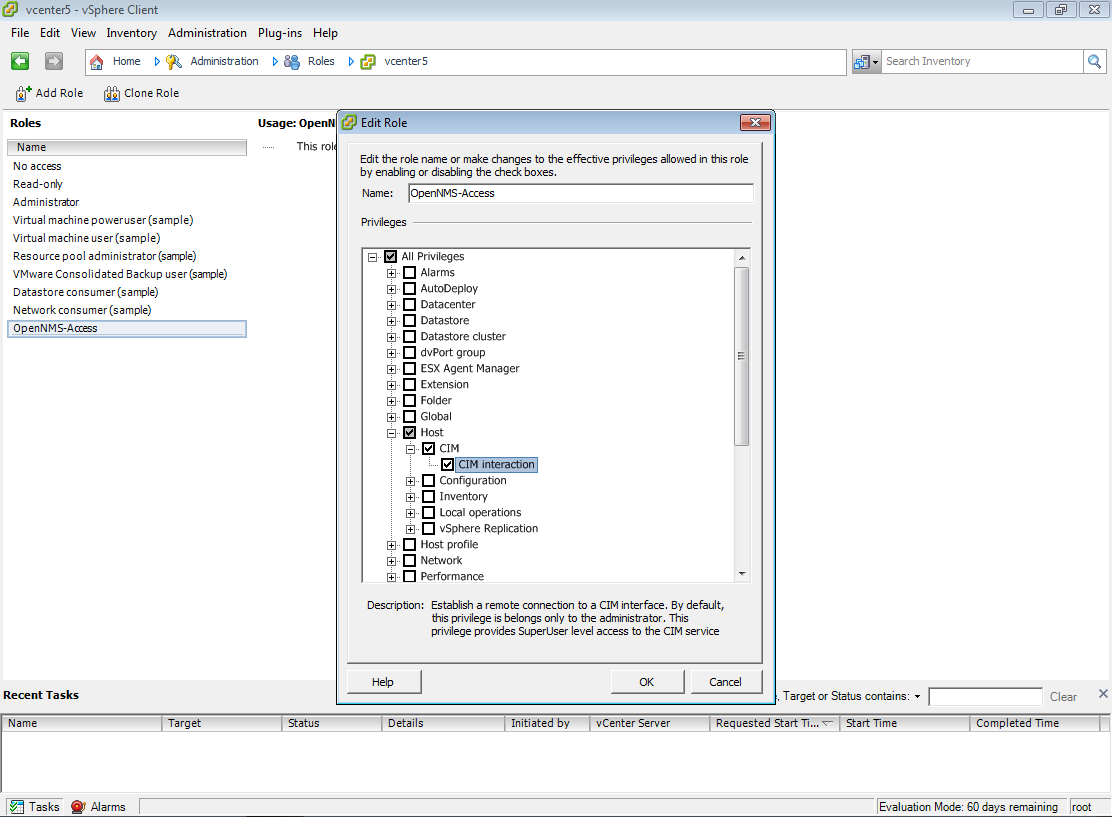
\includegraphics[width=1.0\textwidth]{images/3rd-party/vmware/1-editing}
	\caption{Duplizieren einer \emph{Read-Only} Rolle in \emph{vCenter}}
	\label{pic:vmware-editing}
\end{figure}

\begin{figure}[H]
	\centering
	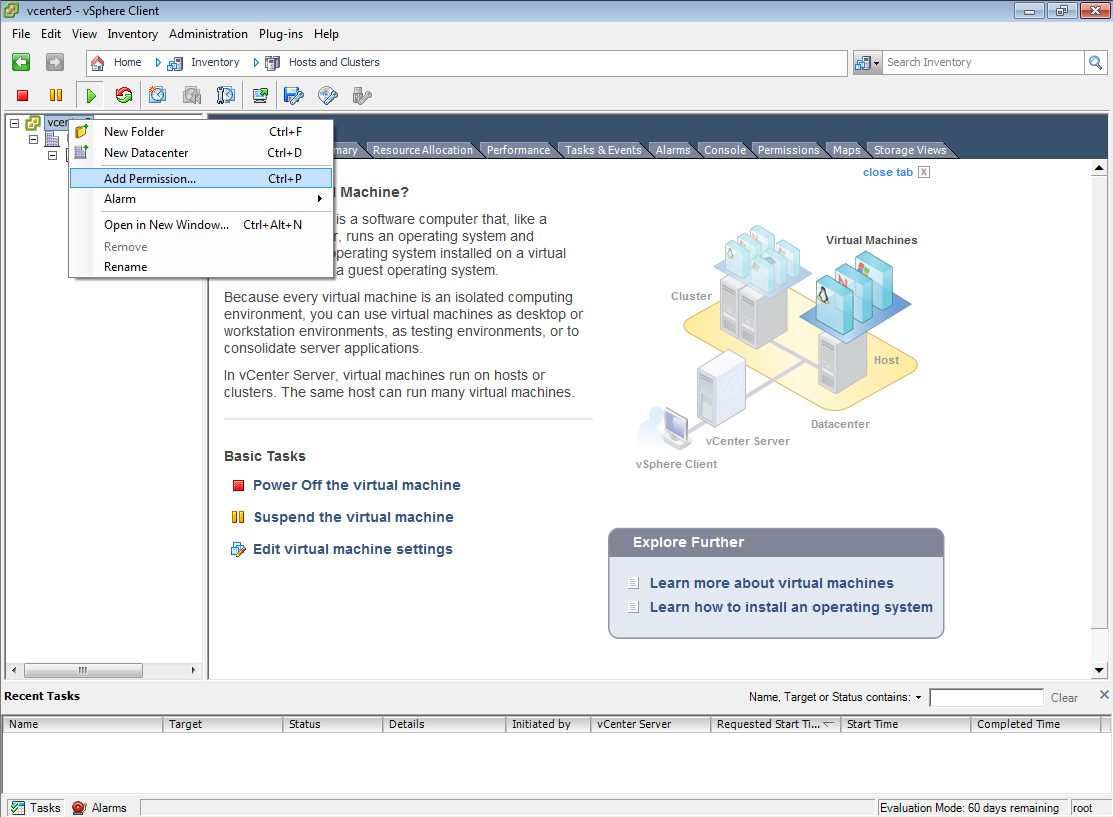
\includegraphics[width=1.0\textwidth]{images/3rd-party/vmware/2-permission}
	\caption{Duplizieren einer \emph{Read-Only} Rolle in \emph{vCenter}}
	\label{pic:vmware-permission}
\end{figure}

\begin{figure}[H]
	\centering
	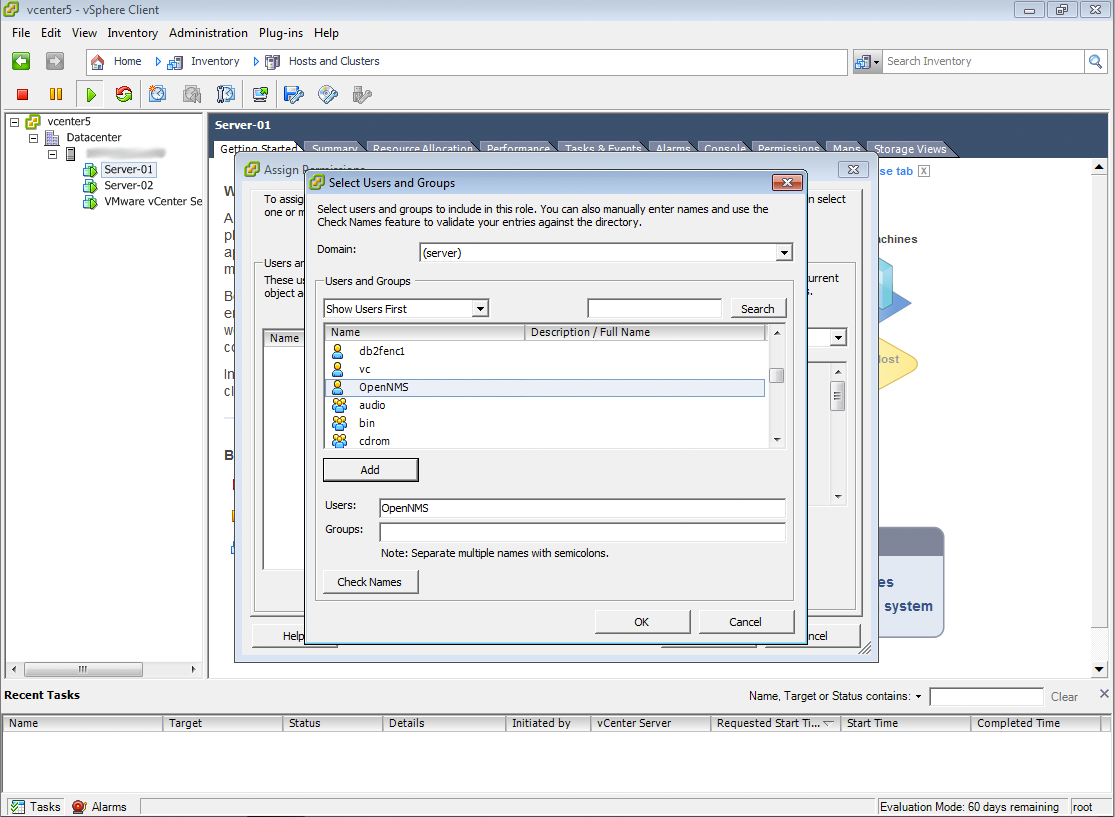
\includegraphics[width=1.0\textwidth]{images/3rd-party/vmware/3-adding}
	\caption{Duplizieren einer \emph{Read-Only} Rolle in \emph{vCenter}}
	\label{pic:vmware-adding}
\end{figure}

\begin{figure}[H]
	\centering
	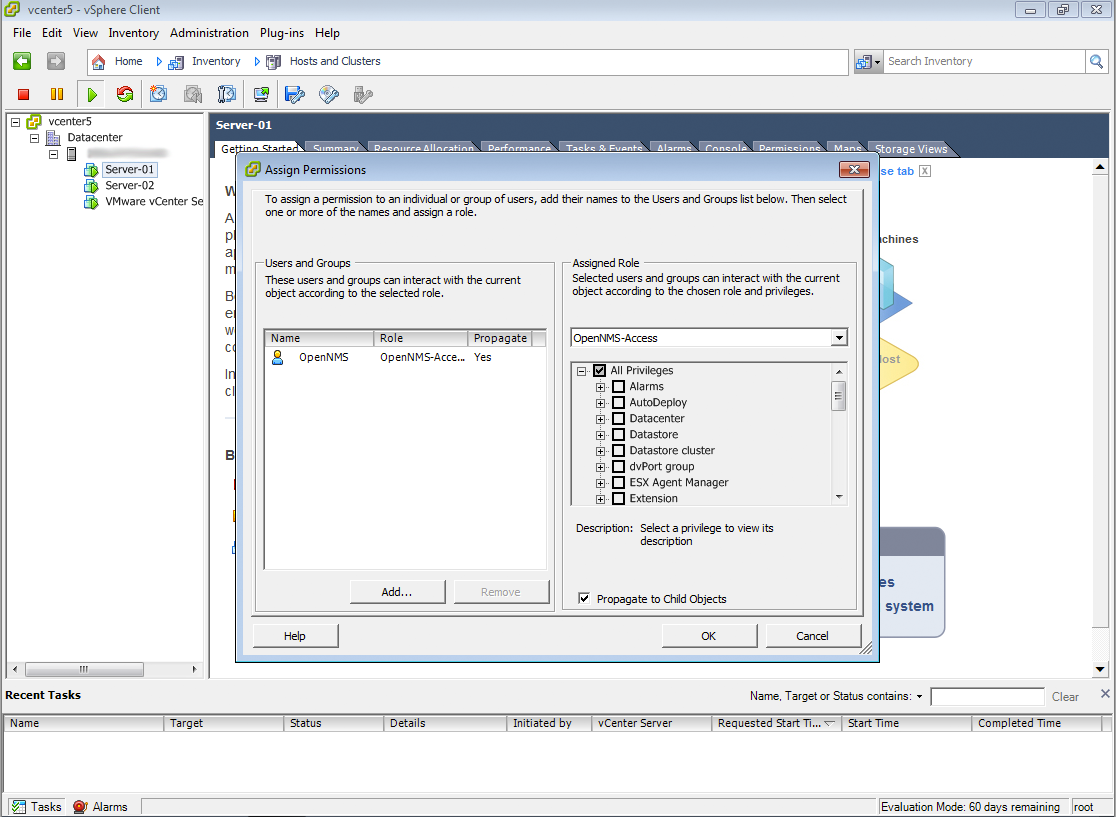
\includegraphics[width=1.0\textwidth]{images/3rd-party/vmware/4-ok}
	\caption{Duplizieren einer \emph{Read-Only} Rolle in \emph{vCenter}}
	\label{pic:vmware-ok}
\end{figure}

\begin{figure}[H]
	\centering
	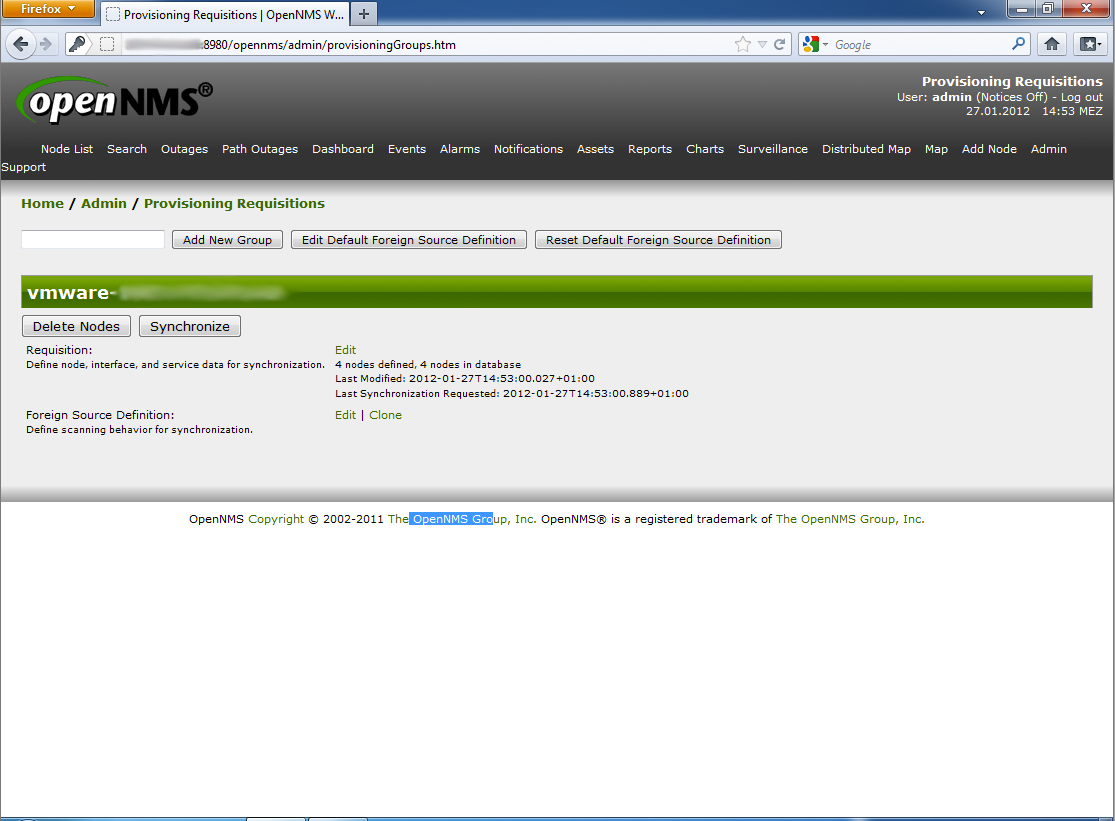
\includegraphics[width=1.0\textwidth]{images/3rd-party/vmware/5-provisioning}
	\caption{Duplizieren einer \emph{Read-Only} Rolle in \emph{vCenter}}
	\label{pic:vmware-provisioning}
\end{figure}

\begin{figure}[H]
	\centering
	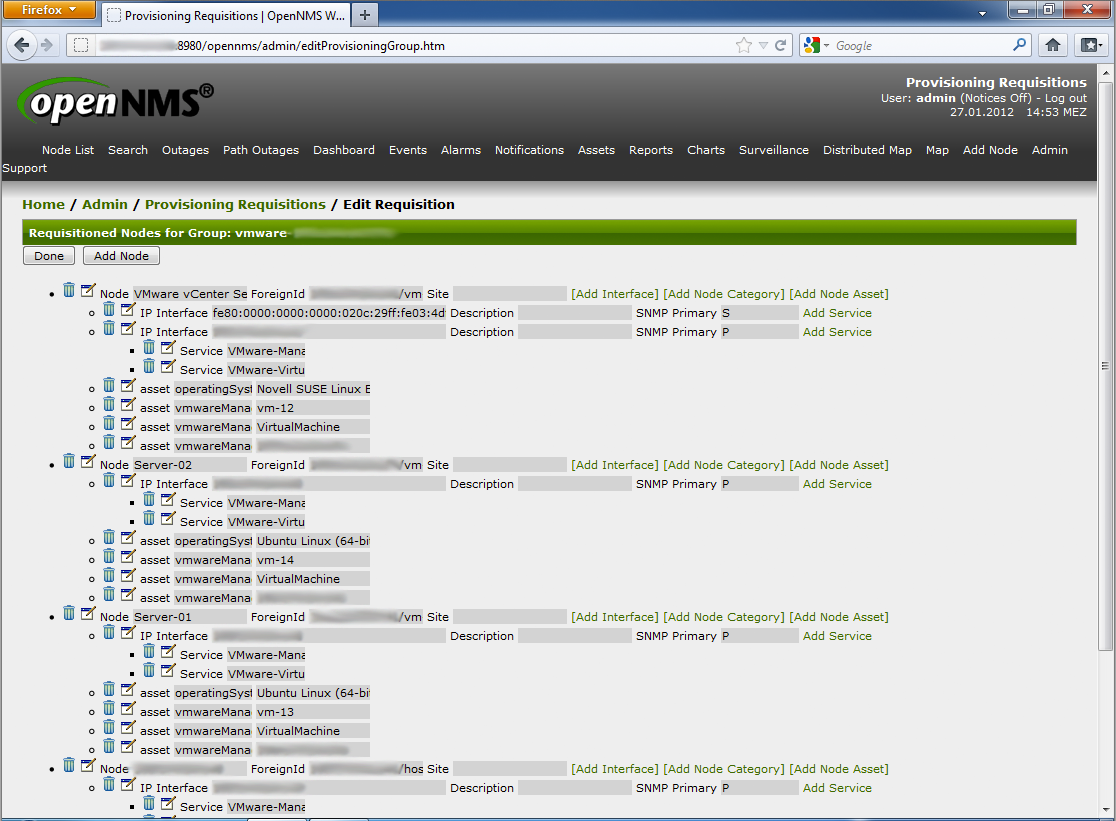
\includegraphics[width=1.0\textwidth]{images/3rd-party/vmware/6-group}
	\caption{Duplizieren einer \emph{Read-Only} Rolle in \emph{vCenter}}
	\label{pic:vmware-group}
\end{figure}

\begin{figure}[H]
	\centering
	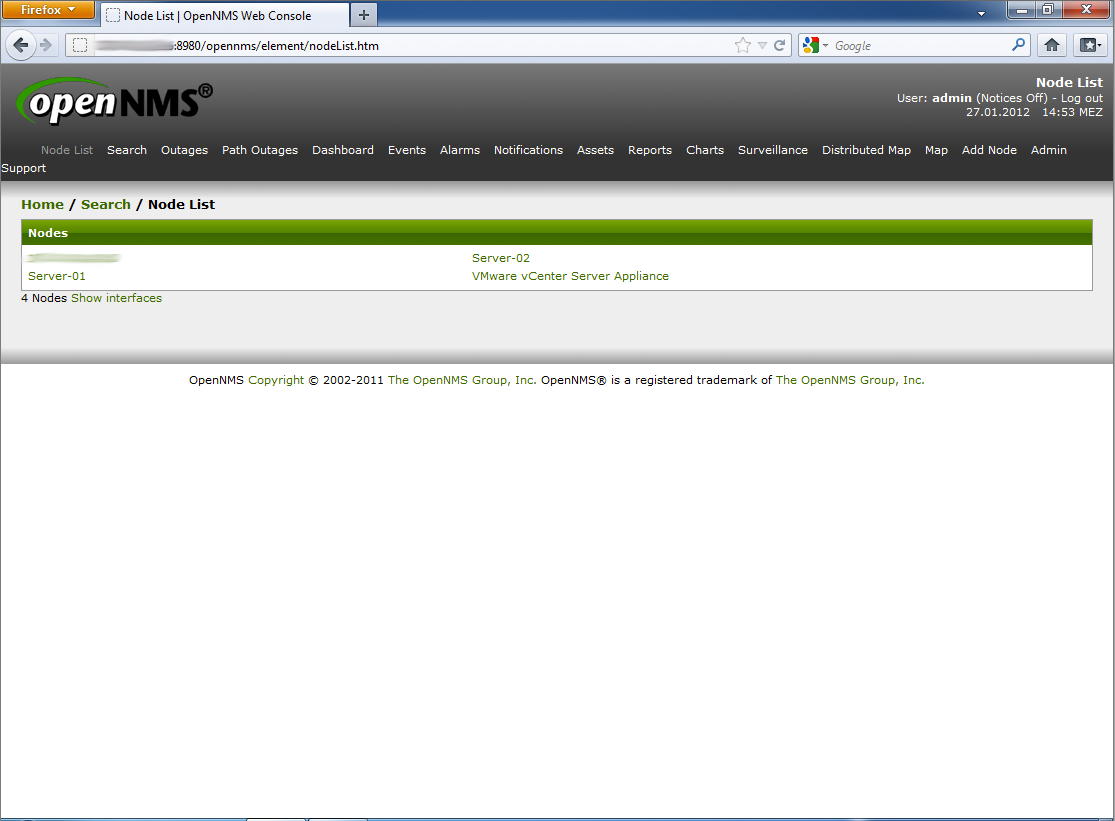
\includegraphics[width=1.0\textwidth]{images/3rd-party/vmware/7-nodes}
	\caption{Duplizieren einer \emph{Read-Only} Rolle in \emph{vCenter}}
	\label{pic:vmware-nodes}
\end{figure}

\begin{figure}[H]
	\centering
	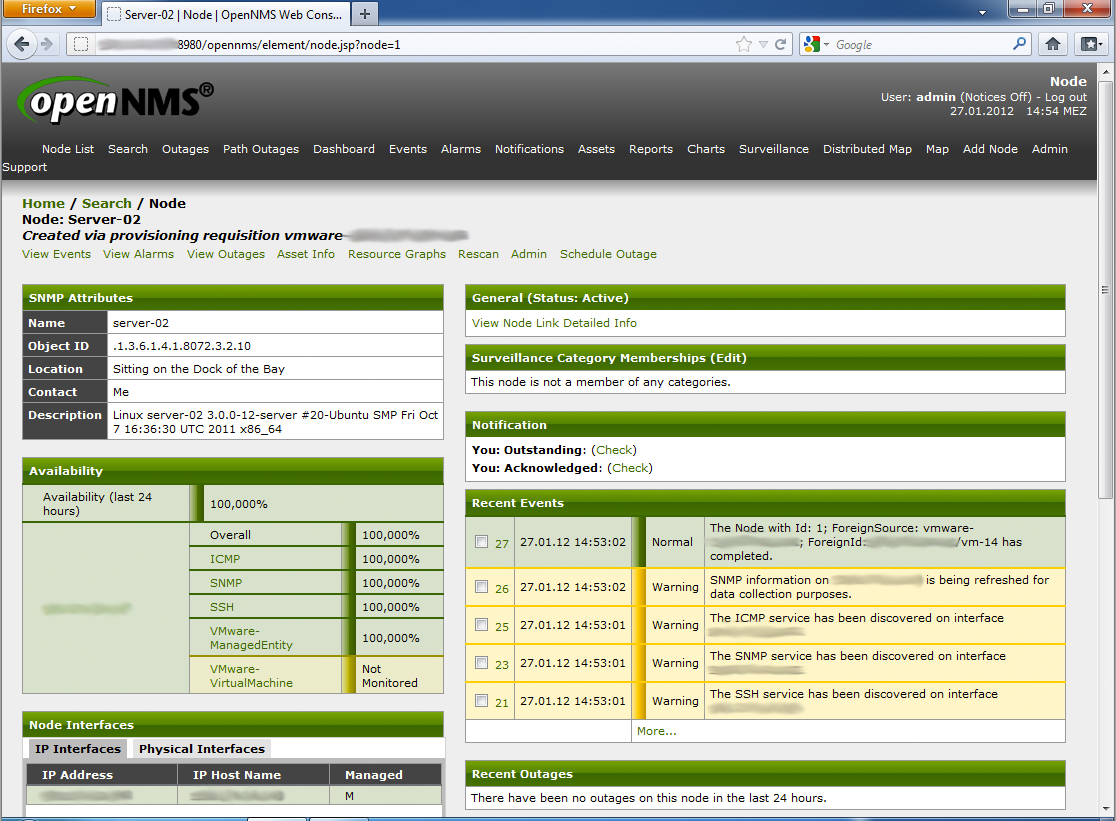
\includegraphics[width=1.0\textwidth]{images/3rd-party/vmware/8-detail}
	\caption{Duplizieren einer \emph{Read-Only} Rolle in \emph{vCenter}}
	\label{pic:vmware-detail}
\end{figure}


%=======================================================
\subsection{VMware Provisioning Adapter}
%=======================================================
In \emph{VMware vCenter} werden alle Komponenten verwaltet, die in der virtuellen Umgebung eingesetzt werden. Dort werden neben den VMs und Host-Systemen auch Leistungsdaten und der Hardwarestatus der Host-Systeme ermittelt und zur Verfügung gestellt. Um die VMs und Host-Systeme von einem bestehenden \emph{vCenter} zu importieren wurde das \emph{Provisioning} um einen \emph{Requisition-Handler} erweitert. Dieser verbindet sich zum \emph{vCenter} und liest dort alle notwendigen Informationen der VMs und Host-Systeme und überführt diese in das \emph{OpenNMS Model} für den Import.

Für den Import werden die folgenden Informationen aus vCenter ausgelesen:
\begin{itemize}
  \item \textit{}
\end{itemize}

\begin{figure}[H]
	\centering
	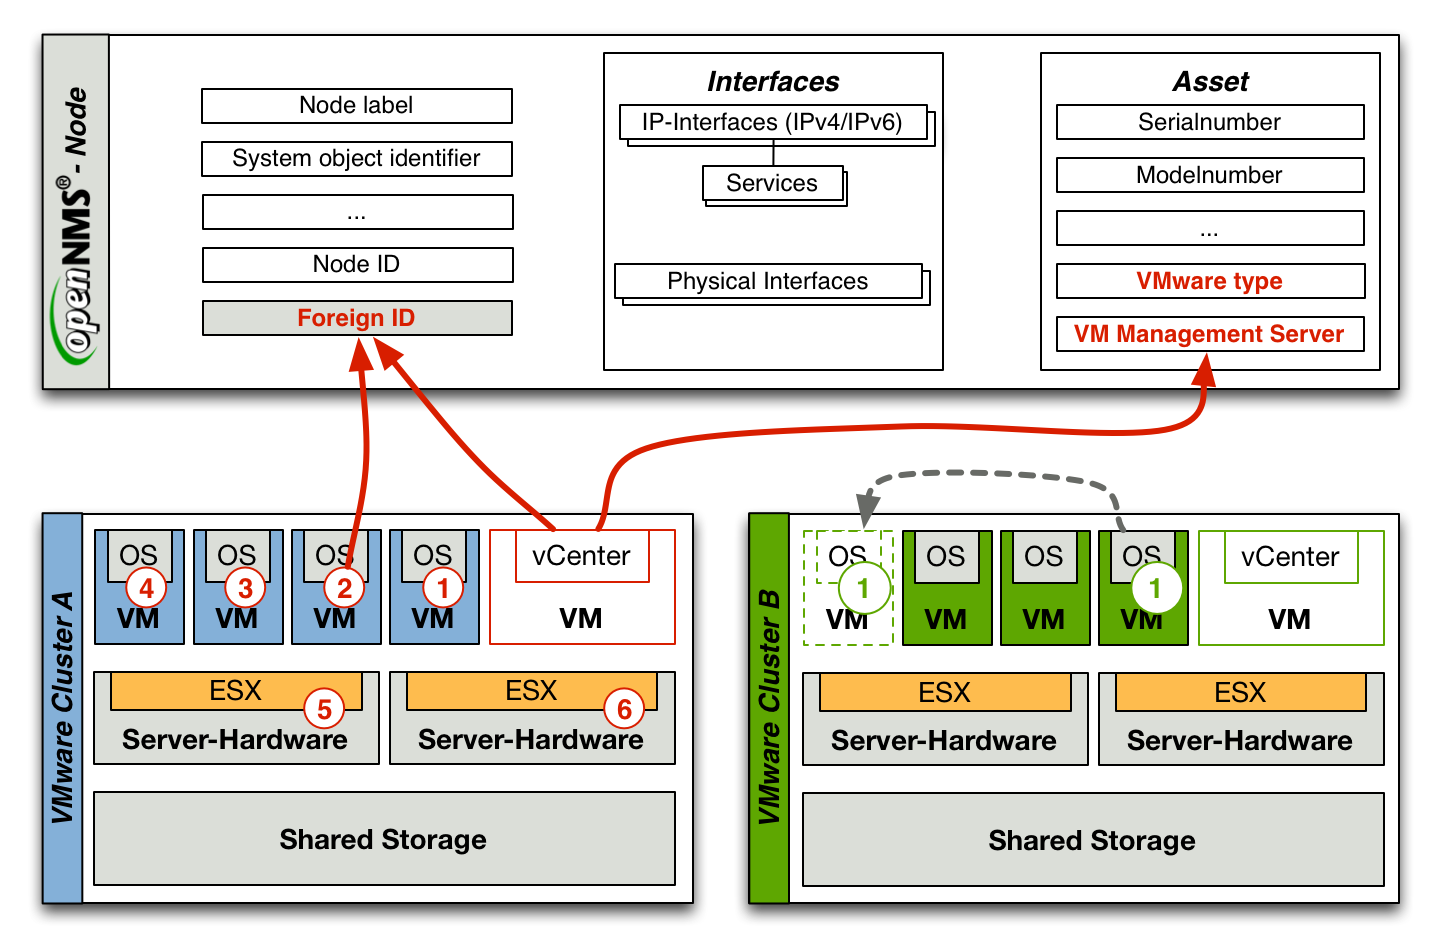
\includegraphics[width=1.0\textwidth]{images/3rd-party/vmware/vmware-cluster}
	\caption{\emph{Provisioning} mit mehreren \emph{VMware Clustern}}
	\label{pic:lab}
\end{figure}


%=======================================================
\subsection{Leistungsdaten von VMware Umgebung}
%=======================================================

%=======================================================
\subsection{Hardwarestatus von VMware Hosts}
%=======================================================

%=======================================================
\subsection{VMware und die Topology Karte}
%=======================================================
%=======================================================
\section{OCS-Inventory Provisioning}
%=======================================================


%=======================================================
\chapter{Anwendungsfälle}
%=======================================================
\epigraphhead[70]{\epigraph{And now for something completely different.}{\textit{Monty Pyton}}}
\include{content/use-cases/introduction}
%=======================================================
\section{Layer 2 - Monitoring}
%=======================================================
Für das Überwachen von Netzwerkverbindungen wird häufig das \textit{ICMP}\footnote{Internet Control Message Protocol zum Test der IP-Konnektivität welches mit dem Kommando \texttt{ping} verwendet wird.} Protokoll der Internetprotokollfamilie verwendet. Es genügt um festzustellen, ob ein Gerät über das Netzwerk noch erreichbar ist oder nicht. Befinden sich redundante Pfade im Netzwerk, kann eine Störung über \textit{ICMP} nicht festgestellt werden, da die \textit{ICMP-Pakete} transparent über einen redundanten Pfad geleitet werden. Die Überwachung wird mit \textit{ICMP} auf der Vermittlungs- oder Netzwerkschicht, also auf \textit{IP-Ebene} durchgeführt. In vielen Fällen werden Fehler oder Statusänderungen auf Basis von \textit{SNMP-Traps}\footnote{SNMP Traps sind Fehlermeldungen die von einer Netzwerkkomponente an einen Managementserver gesendet werden.} übermittelt. Der Status eines Netzwerkports wird beispielsweise mit einem  \textit{Link Down} oder \textit{Link Up} Trap dem Managementserver mitgeteilt.

In vielen Fällen wird entweder ein \textit{SNMP-Trap} für alle oder keinen der  Netzwerkports gesendet. Eine granulare Konfiguration für welchen der Netzwerkports Traps gesendet werden sollen fehlt häufig.

In dem folgenden Versuchsaufbau sollen drei wichtige Switch-Ports überwacht werden. Um festzustellen welche Ports für Monitoring relevant sind, verwenden wir eine benutzerdefinierte \textit{Port-Description}. Als Switch wird ein \textit{Cisco 3524XL} mit \textit{IOS 12.0(5)WC17} verwendet. \textit{OpenNMS} ist in der Version 1.8.1 auf einem \textit{Ubuntu Server 9.10} installiert. Es sind noch keine Geräte in \textit{OpenNMS} eingetragen und es findet noch keine Überwachung statt. Der Versuchsaufbau ist in der folgenden Abbildung dargestellt.

\begin{figure}[H]
	\centering
	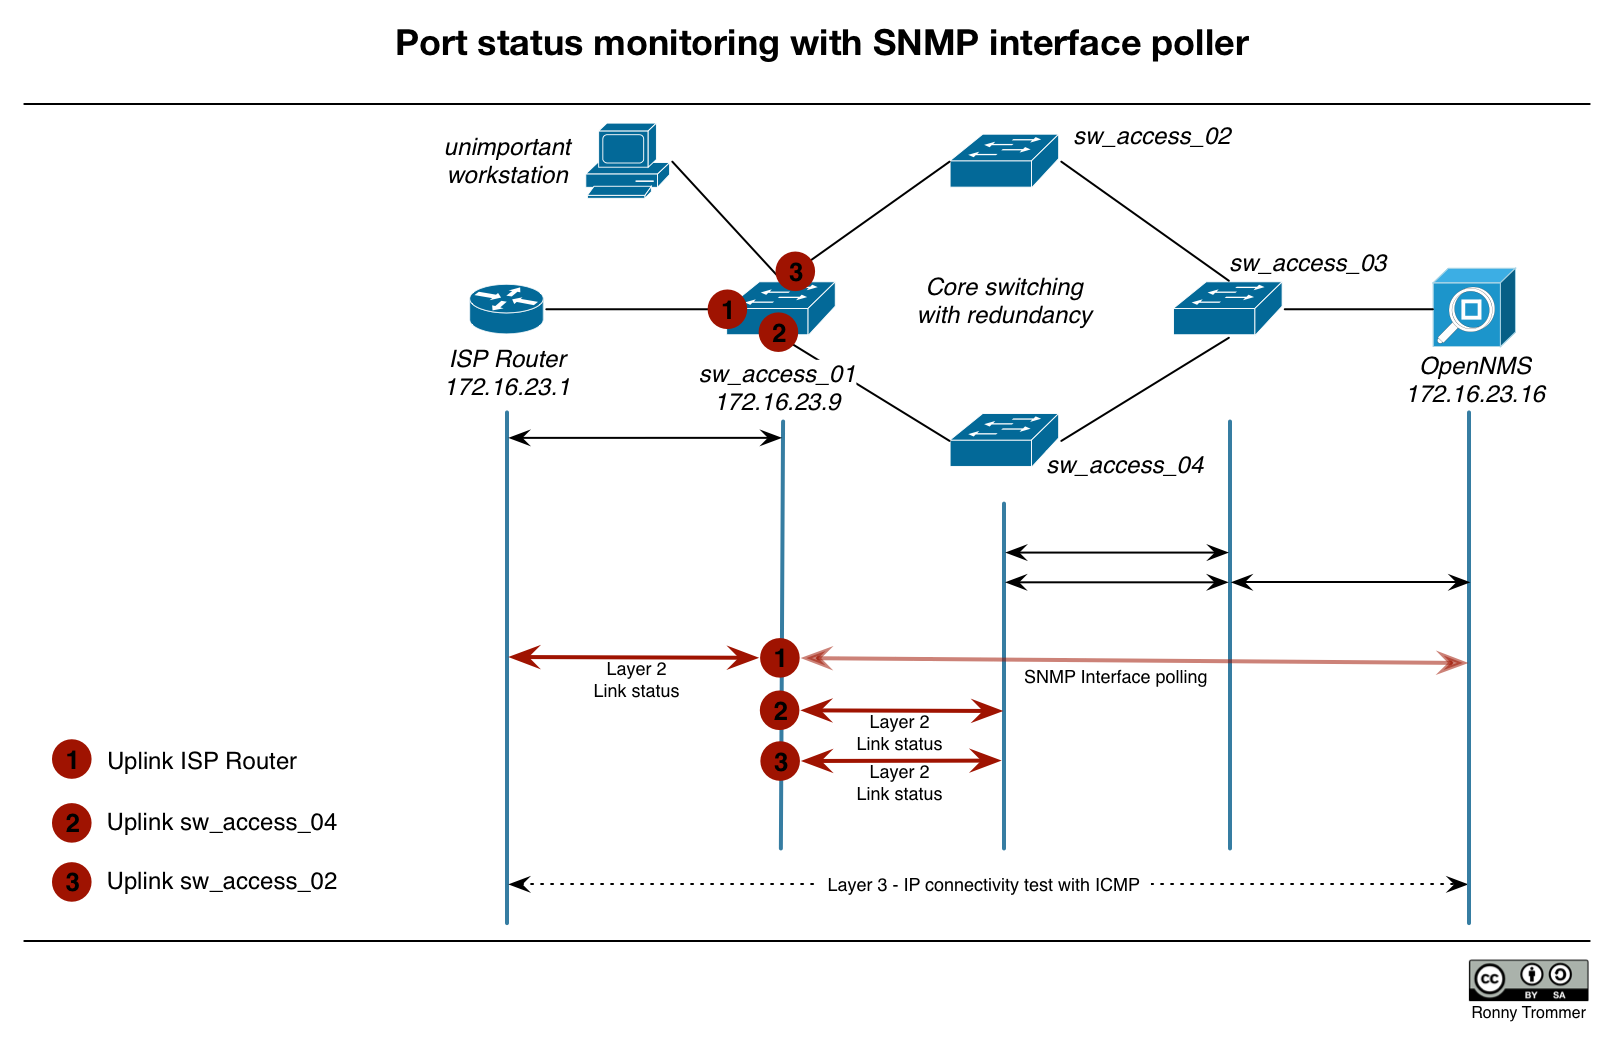
\includegraphics[width=1.0\textwidth]{images/use-cases/monitoring-layer-2/lab-plan}
	\caption{Versuchsaufbau}
	\label{pic:lab}
\end{figure}

Es sollen auf einem Switch mit der Bezeichnung \textit{sw\_access\_01}, drei wichtige Ports überwacht werden. Für die Überwachung relevant ist der Link zum \textit{ISP}\footnote{Internet Service Provider stellt den Übergabepunkt zu Internetdiensten bereit.} Router sowie auch die beiden Uplinks zum redundant ausgelegten Core. Der Port mit der Workstation interessiert uns in der Überwachung nicht und soll entsprechend ignoriert werden. In dem folgendem Versuch wird gezeigt wie \textit{SNMP} auf dem Switch eingerichtet werden kann und in \textit{OpenNMS} aufgenommen wird. Es werden lediglich Leistungsdaten von relevanten Ports aufgezeichnet. Danach wird der \textit{SNMP-Interface Poller} für die entsprechenden Ports eingerichtet.

%=======================================================
\subsection{SNMP-Ready Cisco Switch}
%=======================================================
Bevor wir überhaupt mit der Überwachung anfangen können, muss \textit{SNMP} auf den Geräten eingerichtet werden. Die Einrichtung wird detailiert auf \url{http://www.cisco.com} unter \textit{"Configuring SNMP 3"}\footnote{Configuring SNMP – \url{http://www.cisco.com/en/US/docs/ios/12_2/configfun/configuration/guide/fcf014.html}} beschrieben. Es werden hier nur die rudimentären Schritte zur Einrichtung von \textit{SNMP} beschrieben. Die grundlegende Einrichtung von Authentifizierung, Hostnamen sowie IP-Adressen ist bereits vorgenommen. Wir melden uns per \textit{Telnet} auf unserem Switch an und aktivieren \textit{SNMP} im \textit{Read-Only} Modus und setzen eine \textit{location} und einen \textit{contact}.

\lstinputlisting[caption={SNMP-Konfiguration auf Cisco Switch}
      \label{lst:cisco-snmp-config}]
  {configs/use-cases/monitoring-layer-2/cisco-snmp.cfg}

Damit ist es nun möglich vom \textit{OpenNMS-Server} \textit{SNMP} Abfragen durchzuführen. Im Anschluss werden die entsprechenden \textit{Port-Description} gesetzt.

\lstinputlisting[caption={Konfiguration der Netzwerk-Ports}
       \label{lst:cisco-port-config}]
  {configs/use-cases/monitoring-layer-2/cisco-ports.cfg}

\textbf{\textit{Hinweis:}} Es ist häufig sinnvoll, mit Hilfe von \textit{Access Listen}, Zugriffe nur von IP-Adressen des Management-Servers zu gestatten. Schauen Sie sich hier die entsprechenden \textit{ACLS} an.

Um die SNMP Konfiguration zu testen, können die gesetzten Beschreibungen mit dem Kommando

\begin{lstlisting}[numbers=none]
snmpwalk -v 2c -c notpublic 172.16.23.9 IF-MIB::ifAlias
\end{lstlisting}

vom \textit{OpenNMS-Server} abgerufen werden. Die Ausgabe sollte dann in etwa so aussehen:

\lstinputlisting[caption={\textit{SNMP walk} für die Anzeige der \textit{Port-Description}}
       \label{lst:cisco-ifalias-snmpwalk}]
  {configs/use-cases/monitoring-layer-2/cisco-ifalias-snmpwalk.txt}

Damit sind die Voraussetzungen für das Monitoring in OpenNMS erfüllt und wir können den Switch in OpenNMS für die Überwachung eintragen.

%=======================================================
\subsection{Cisco Switch Provisioning}
%=======================================================
Bevor wir Geräte eintragen, sollte die verwendete \textit{SNMP-Community} bekannt sein. Hierzu gibt es zwei Möglichkeiten, entweder die \textit{default SNMP-Community} ist in der Datei
\begin{lstlisting}[numbers=none]
$OPENNMS_HOME/etc/snmp-config.xml
\end{lstlisting}
entsprechend setzen oder die \textit{Community} wird für die einzelne IP-Adresse oder einen IP-Bereich über die Web-Oberfläche gesetzt. Um die \textit{SNMP-Community} für unseren Switch mit der IP 172.16.23.9 zu setzen, wird das Formular in der Web-Oberfläche wie folgt ausgefüllt.
\begin{lstlisting}[numbers=none]
Admin --> Configure SNMP Community Names by IP
\end{lstlisting}
\begin{figure}[H]
	\centering
	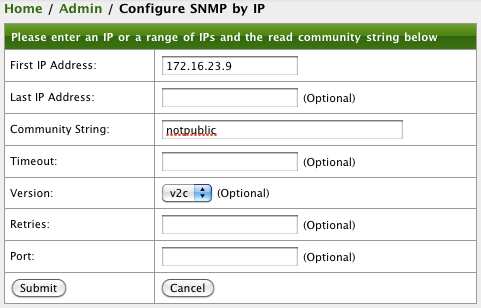
\includegraphics[width=1.0\textwidth]{images/use-cases/monitoring-layer-2/configure-snmp-by-ip}
	\caption{SNMP Community für IP-Adressen konfigurieren}
	\label{pic:configure-snmp-by-ip}
\end{figure}
Im nächsten Schritt wird der Switch über das \textit{Provisioning} von \textit{OpenNMS} aufgenommen. Wir erzeugen eine neue \textit{Requisition Group} über 
\begin{lstlisting}[numbers=none]
Admin --> Manage Provisioning Groups --> Add New Group
\end{lstlisting}
mit der Bezeichnung \textit{OpenNMS Lab}. Wir erstellen eine \textit{Policy}\footnote{\textit{Policies} beschreiben Richtlinien für das Monitoring in \textit{OpenNMS} und werden während des Import in die \textit{OpenNMS-Datenbank} angewendet.} die nur Leistungsdaten von relevanten und aktiven Ports aufzeichnet. Zusätzlich soll nur \textit{ICMP} und \textit{SNMP} für den Switch überwacht werden. Die \textit{Policy} sieht dazu wie folgt aus:
\begin{figure}[H]
	\centering
	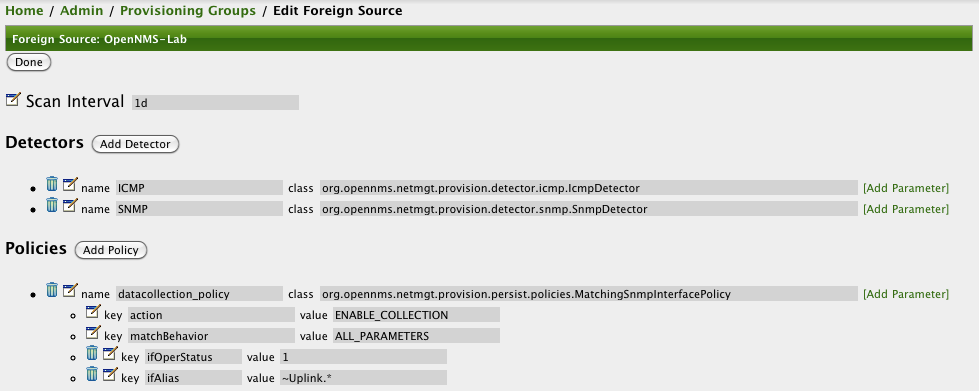
\includegraphics[width=1.0\textwidth]{images/use-cases/monitoring-layer-2/requisition-policy}
	\caption{Richtlinie für den Import des \textit{Cisco} Switch}
	\label{pic:requisition-policy}
\end{figure}
Alle Detektoren ausser \textit{ICMP} und \textit{SNMP} wurden entfernt. Zusätzlich wurde eine \textit{datacollection\_policy} angelegt, die nur Leistungsdaten von Ports aufzeichnet, welche aktiv sind und\footnote{Die Verknüpfung stammt aus dem Konfigurationsschlüssel \textit{matchBehavior}, \textit{oder=ANY\_PARAMETER}, \textit{Negation=NON\_PARAMETERS}} eine Port-Beschreibung\footnote{In der \textit{SNMP MIB II} ist \textit{ifDescr} die Interface-Bezeichnung \textit{(FastEthernet 0/1)} und der \textit{ifAlias} die Port Beschreibung} mit \textit{Uplink} beginnend besitzen. Die Geräte in der \textit{Requisition Group} wird täglich\footnote{Definiert über den Standardparameter \textit{Scan Interval 1d}} einmal synchronisiert. Der Switch wird nun unter 
\begin{lstlisting}[numbers=none]
Requisition (Provisioning Group): EDIT --> Add Node
\end{lstlisting}
eingetragen und synchronisiert.
\begin{figure}[H]
	\centering
	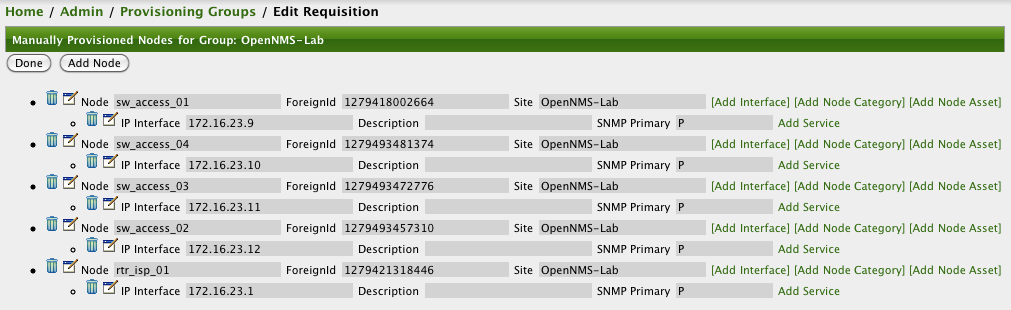
\includegraphics[width=1.0\textwidth]{images/use-cases/monitoring-layer-2/requisition-import}
	\caption{Import der \textit{Requisition Group} in \textit{OpenNMS}}
	\label{pic:requisition-import}
\end{figure}
Die Konfiguration wird bestätigt, über die Schaltfläche \textit{Synchronize} importiert und im Monitoring bereitgestellt. Nach dem Import stellt sich der Switch in OpenNMS wie folgt dar:
\begin{figure}[H]
	\centering
	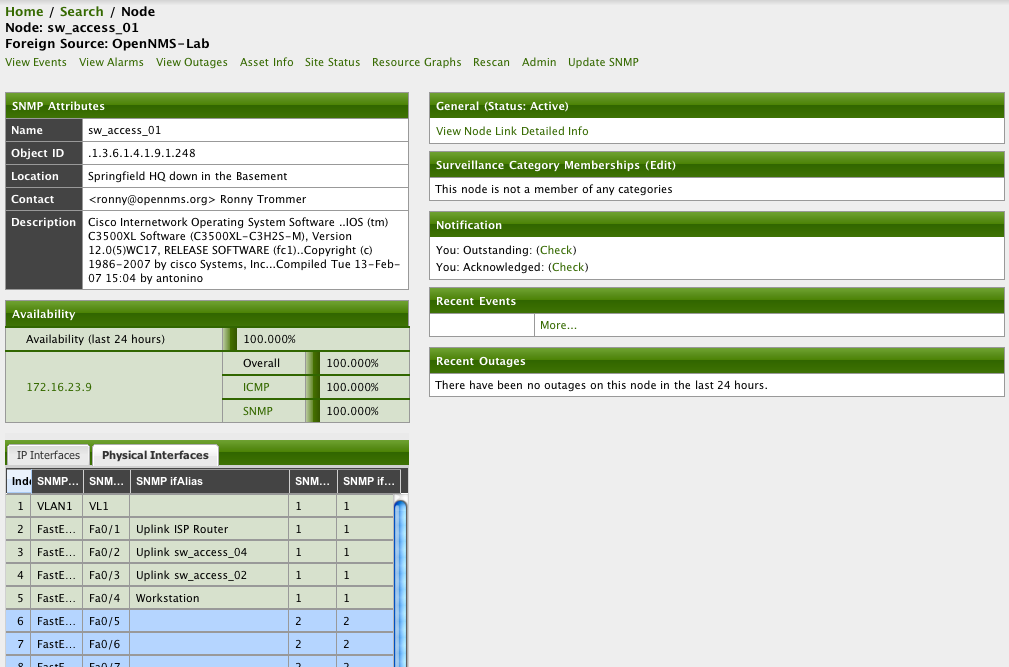
\includegraphics[width=1.0\textwidth]{images/use-cases/monitoring-layer-2/node-page}
	\caption{\textit{Node Page} des Cisco-Switch nach dem Import in \textit{OpenNMS}}
	\label{pic:node-page}
\end{figure}
Zur besseren Darstellung wurden die Spalten mit der Interface-Geschwindigkeit und IP-Adresse ausgeblendet und der \textit{Port-Status} hinzugefügt. Die grün hinterlegten Ports sind aktiv. Die blau hinterlegten Ports sind administrativ deaktiviert. Der Switch wird nun täglich  mit den entsprechenden Port-Beschreibungen in OpenNMS synchronisiert und die entsprechenden Informationen im Monitoring bereitgestellt. Es werden zusätzlich nur Leistungsdaten von Ports mit der Beschreibung \textit{Uplink} aufgezeichnet.
\begin{figure}[H]
	\centering
	\includegraphics[width=1.0\textwidth]{images/use-cases/monitoring-layer-2/uplink-datacollection}
	\caption{Leistungsdaten werden nur von Ports mit der Beschreibung \textit{Uplink} gesammelt.}
	\label{pic:uplink-datacollection}
\end{figure}

%=======================================================
\subsection{Port Status kontrollieren}
%=======================================================
Zu Begin muss der dazu verwendete \textit{SNMP Interface Poller} aktiviert werden. In der Datei
\begin{lstlisting}[numbers=none]
$OPENNMS_HOME/etc/service-configuration.xml
\end{lstlisting}
wird dazu der entsprechende Dienst auskommentiert.
\lstinputlisting[language=XML, caption={Der \textit{SNMP Interface Poller} ist nach der Installation von \textit{OpenNMS} einkommentiert.}
       \label{lst:opennms-service-ifpoller}]
  {configs/use-cases/monitoring-layer-2/opennms-service-config.xml}
Im nächsten Schritt wird ein \emph{Interface Polling Package} angelegt. In diesem wird festgelegt, welche Ports zu überwachen sind.
\begin{lstlisting}[numbers=none]
vi $OPENNMS_HOME/etc/snmp-interface-poller-configuration.xml
\end{lstlisting}
Die package-Beschreibung wird wie folgt aufgebaut:
\lstinputlisting[language=XML, caption={\textit{Polling-Package} für den \textit{SNMP-Interface Poller}}
       \label{lst:opennms-ifpoller-package}]
  {configs/use-cases/monitoring-layer-2/snmp-interface-poller-package-config.xml}
Damit nur Ports mit der Beschreibung \textit{Uplink} überwacht werden, wird ein Filterkritierum angegeben. Dieses lässt sich logisch mit weiteren Kriterien mit \textit{AND} und \textit{OR} verknüpfen. Mit \textit{snmpifalias like 'Uplink\%'} wird der entsprechende \textit{Alias} aus der Datenbank ausgelesen und überwacht. Der Port Status wird alle 5 Minuten getestet und aktualisiert. Es können als Bedingung alle Felder aus der Tabelle \textit{snmpinterface} verwendet werden. In der Version 1.8.1 sind folgende Spalten verwendbar:

\pagebreak

\begin{longtable}{|p{3.5cm}|p{11cm}|}
  % Kopf auf erste Seite
  \hline
    \rowcolor{light_gray}[5.8pt]
 	 Bezeichnung	&	Beschreibung \\
	 \hline
	 \endfirsthead
	 %Kopf auf weiteren Seiten
	 \hline \multicolumn{2}{|c|}{(Fortsetzung)}\\
	 \hline
	 \rowcolor{light_gray}[5.8pt]
	 Bezeichnung	&	Beschreibung \\
	 \hline
	 \endhead
	 \hline
	 \multicolumn{2}{|c|}{(Tabelle wird auf der nächsten Seite fortgesetzt)}
  \endfoot
  \hline
	\caption{Verwendbare Attribute der SNMP interface table}
  \endlastfoot
	\hline
  	nodeid    &    Eindeutige ID für den Knoten in OpenNMS. \\
  	\hline
  	ipaddr    &    RFC-1213-MIB: The media-dependent physical address. Setting this object to a null string (one of zero length) has the effect of invaliding the corresponding entry in the atTable object.  That is, it effectively dissasociates the interface identified with said entry from the mapping identified with said entry.  It is an implementation-specific matter as to whether the agent removes an invalidated entry from the table. Accordingly, management stations must be prepared to receive tabular information from agents that corresponds to entries not currently in use. Proper interpretation of such entries requires examination of the relevant atPhysAddress object. \\
  	\hline
  	snmpipadentnetmask    &    RFC1213-MIB: The NetworkAddress (e.g., the IP address) corresponding to the media-dependent `physical' address. \\
  	\hline
  	snmpphysaddr    &    RFC-1213-MIB: The interface's address at the protocol layer immediately `below' the network layer in the protocol stack.  For interfaces which do not have such an address (e.g., a serial line), this object should contain an octet string of zero length. \\
  	\hline
  	snmpifdescr    &    RFC-1213-MIB: A textual string containing information about the interface.  This string should include the name of the manufacturer, the product name and the version of the hardware interface. \\
  	\hline
  	snmpiftype    &    RFC-1213-MIB (Nur ein Auszug): Interface type
other(1), ethernetCsmacd(6), basicISDN(20), primaryISDN(21), propPointToPointSerial(22), ppp(23),softwareLoopback(24), frameRelay(32), atm(37), aal5(49), isdn(63), adsl(94), sdsl(96), vdsl(97), pppMultilinkBundle(108), atmVirtual(149),mplsTunnel(150), mpls166), adsl2(230), adsl2plus(238)
RFC-1213-MIB: The type of interface, distinguished according to the physical/link protocol(s) immediately `below' the network layer in the protocol stack. \\
    \hline
    snmpifname    &    Bei Cisco Kurzbezeichnung Fa/0/2 \\
    \hline
    snmpifspeed    &    RFC-1213-MIB:  An estimate of the interface's current bandwidth in bits per second.  For interfaces which do not vary in bandwidth or for those where no accurate estimation can be made, this object should contain the nominal bandwidth. \\
    \hline
    snmpifadmin    &    Administrativer Status: up(1), down(2), testing(3)
RFC-1213-MIB: The desired state of the interface.  The testing(3) state indicates that no operational packets can be passed. \\
    \hline
    snmpifoperstatus    &    Operativer Status: up(1), down(2), unknown(4), dormant(5), notPresent(6), lowerLayerDown(7)
RFC-1213-MIB: The current operational state of the interface. The testing(3) state indicates that no operational packets can be passed. \\
    \hline
    snmpifalias    &    Eigene Port Beschreibung \\
    \hline
    snmpcollect    &    (N) Not Collect oder (C) Collect.Gibt an ob Leistungsdaten aufgezeichnet werden sollen oder nicht.
    \label{tbl:snmpifattrib}
\end{longtable}

Die vollständige Konfigurationsdatei wird im folgenden komplett dargestellt.

\lstinputlisting[language=XML, caption={SNMP Interface Poller konfiguration.}
       \label{lst:opennms-ifpoller-configuration}]
  {configs/use-cases/monitoring-layer-2/snmp-interface-poller-config.xml}

Damit die Einstellung wirksam werden, muss OpenNMS neu gestartet werden.
\begin{lstlisting}[numbers=none]
service opennms restart
\end{lstlisting}

%=======================================================
\subsection{Funktionstest}
%=======================================================
Im nächsten Schritt prüfen wir das Verhalten von OpenNMS wenn verschiedene Ports den Status ändern. Dazu werden zwei Testszenarien geprüft:
\begin{enumerate}
\item{Ein Uplink Port und der Workstation Port werden abgezogen und ein Ausfall simuliert. Es sollte nur ein Port Down Event auf dem Uplink Port erzeugt werden.}
\item{Ein Uplink Port und der Workstation Port werden administrativ down gesetzt. Zusätzlich simulieren wir eine echte Störung auf dem Uplink zum ISP-Router.}
\end{enumerate}
In der Ausgangssituation läuft alles wie gewünscht. Alle Ports sind aktiv und funktionsbereit.
\begin{figure}[H]
	\centering
	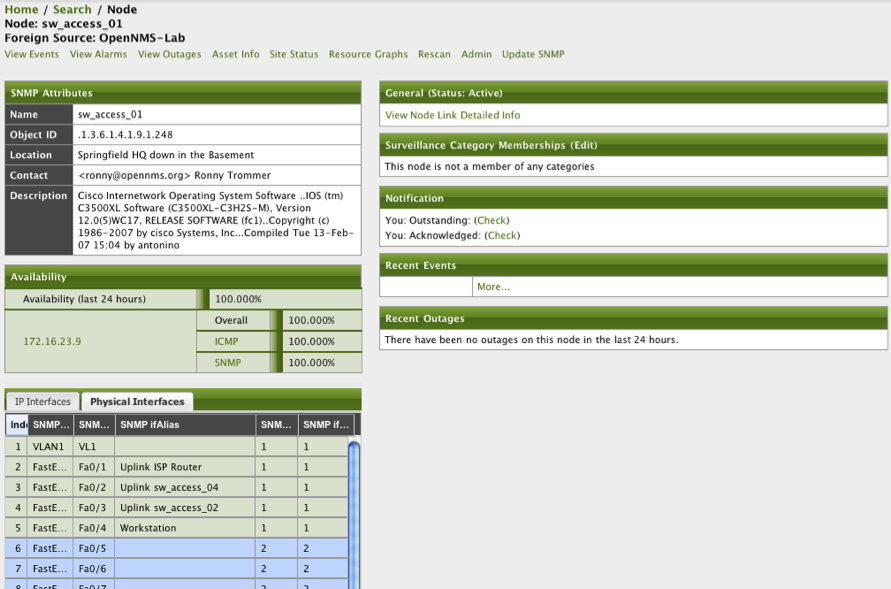
\includegraphics[width=1.0\textwidth]{images/use-cases/monitoring-layer-2/node-page-snmpifpoller}
	\caption{Node page mit Port status für \emph{Physical Interfaces}.}
	\label{pic:node-page-snmpifpoller}
\end{figure}

%=======================================================
\subsubsection{Szenario 1: Port Störungen}
%=======================================================
Die Ports \emph{Fa0/3} und \emph{Fa0/4} wurden abgezogen und simulieren einen Ausfall. Wir sehen, dass der Portstatus nur für den Port \emph{Fa0/3} aktualisiert wurde.
\begin{figure}[H]
	\centering
	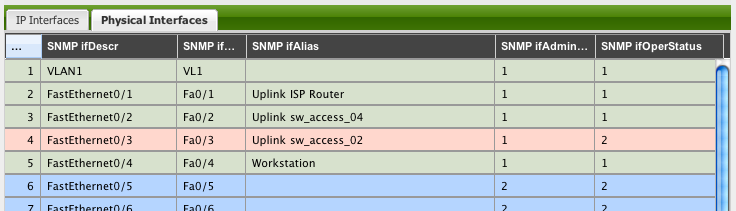
\includegraphics[width=1.0\textwidth]{images/use-cases/monitoring-layer-2/port-outage}
	\caption{Anzeige Port Störung eines \emph{Physical Interfaces}.}
	\label{pic:port-outage-snmpifpoller}
\end{figure}
OpenNMS erzeugt zusätzlich ein entsprechendes Event und protokolliert damit das Ereignis.
\begin{figure}[H]
	\centering
	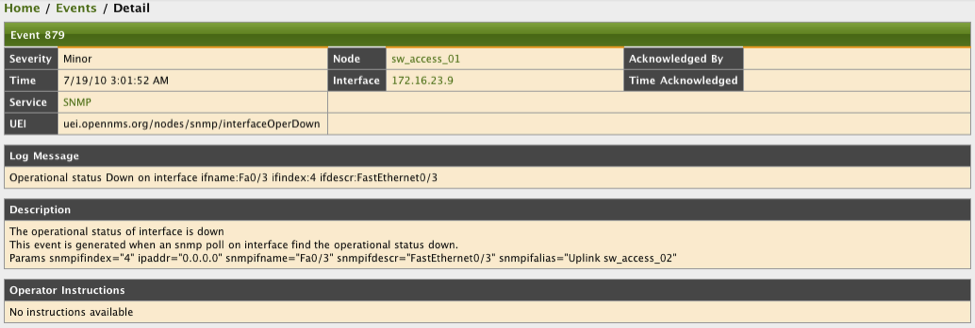
\includegraphics[width=1.0\textwidth]{images/use-cases/monitoring-layer-2/port-down-event}
	\caption{\emph{Event} bei Port-Störung.}
	\label{pic:port-down-event}
\end{figure}
Der Status des Ports \emph{Fa0/4} wird nicht durch den \emph{SNMP-Interface Poller} aktualisiert. Es wurde ja explizit angegeben, dass nur \emph{Uplink} Ports überwacht werden. Erst bei einer neuen Synchronisation der kompletten \emph{Provisioning Group} wird auch der entsprechende Port-Status der Workstation wieder mit übernommen. Das Interval beträgt einen Tag. Wir synchronisieren manuell und der entsprechende Port Status wird wie folgt angzeigt.
\begin{figure}[H]
	\centering
	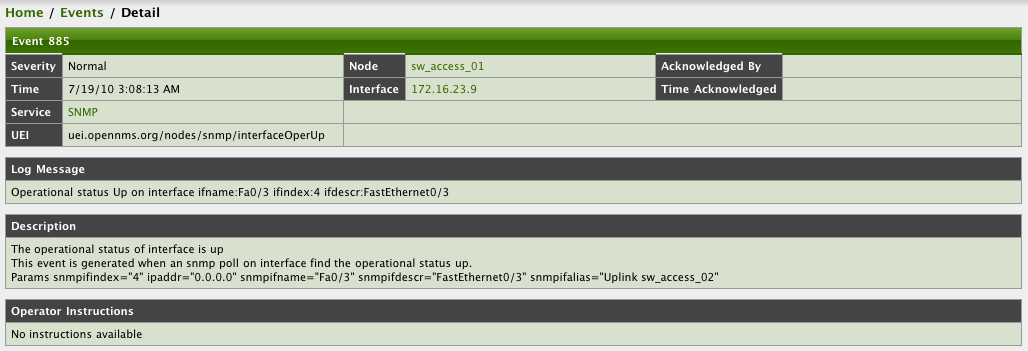
\includegraphics[width=1.0\textwidth]{images/use-cases/monitoring-layer-2/port-up-event}
	\caption{\emph{Event} beim auflösen der Port-Störung.}
	\label{pic:port-up-event}
\end{figure}
Damit ist der erste Testfall erfolgreich abgeschlossen. Im zweiten Testfall prüfen wir, ob der Administrative Status korrekt überwacht wird.

%=======================================================
\subsubsection{Szenario 2: Störung und administrativ deaktiviert}
%=======================================================
Wir gehen wie gehabt von einem voll funktionsfähigem Netzwerk aus. Alle Ports sind aktiv und funktionsbereit. Es werden nun wiederum zwei Ports manuell deaktiviert8. Der Status sieht nun wie folgt aus.
\begin{figure}[H]
	\centering
	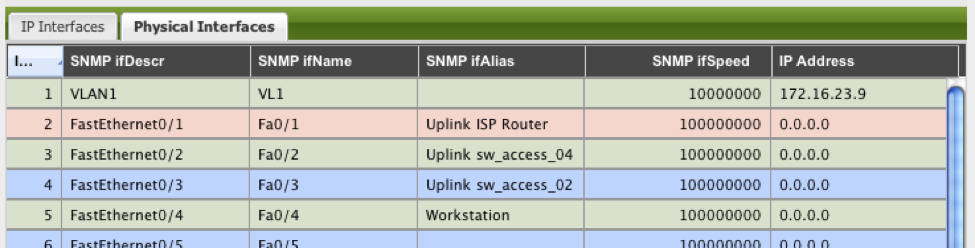
\includegraphics[width=1.0\textwidth]{images/use-cases/monitoring-layer-2/port-admin-down}
	\caption{Interface status nach administrativen deaktivieren des Ports.}
	\label{pic:port-admin-down}
\end{figure}
Wir erhalten zwei unterschiedliche Meldungen und zwar über den Port \emph{Fa0/1} sowie \emph{Fa0/3}. Der Port \emph{Fa0/4} für die Workstation wird komplett ignoriert. Für den administrativen Status wird ein eigenes Event \emph{interfaceAdminDown} erzeugt.
\begin{figure}[H]
	\centering
	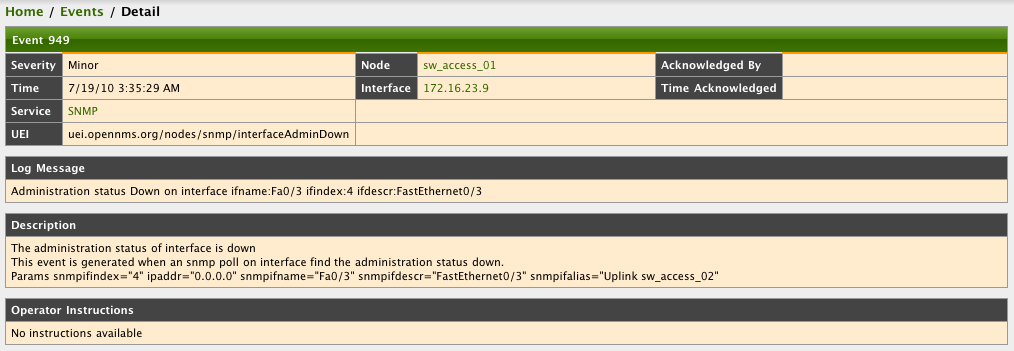
\includegraphics[width=1.0\textwidth]{images/use-cases/monitoring-layer-2/port-admin-down-event}
	\caption{\emph{Event} nach dem administrativen deaktivieren des Ports.}
	\label{pic:port-admin-down-event}
\end{figure}
Bei einer echten Störung wird ein Event \emph{interfaceOperDown} generiert. Damit ist der Funktionstest abgeschlossen und auf die entsprechenden Events können verschiedene Benachrichtigungen eingerichtet werden. Für die Benachrichtigung stehen die folgenden Events zur Verfügung
\begin{itemize}
  \item{Snmp Interface Admin Status Down}
  \item{Snmp Interface Admin Status Up}
  \item{Snmp Interface Oper Status Down}
  \item{Snmp Interface Oper Status Up}
\end{itemize}
Damit sollte einer Port Status Überwachung in OpenNMS nichts mehr im Wege stehen. 
%=======================================================
\section{Monitoring mit Skripten}
%=======================================================
Für die Überwachung von speziellen Anwendungen oder Arbeitsabläufen, reichen bestehende standardisierte Managementagenten häufig nicht aus. Die notwendigen Statusinformationen können über Standard- oder Herstellerspezifische \emph{SNMP\footnote{SNMP ist das Simple Network Management Protocol} MIB}\footnote{Management Information Base} nicht abgefragt werden. Um hier spezielle Anforderungen erfüllen zu können ist es möglich eigene Programme oder Skripte zur Überwachung einzubinden. Um ein möglichst praxisnahes und durchgängiges Beispiel liefern zu können, konfigurieren wir exemplarisch eine Festplattenüberwachung mit \emph{S.M.A.R.T}\footnote{Self-Monitoring, Analysis and Reporting Technology}. Um die Abläufe zu verdeutlichen richten wir einen  Monitor ein, der den Zustand einer lokal installieren Festplatte überwacht.

Die Verwendung der eigenen Programme und Skripte kann auf unterschiedliche Art und Weise realisiert werden. Im ersten Teil wird beschrieben, wie der unter \emph{Unix/Linux} weit verbreitete \emph{Net-SNMP} Agent erweitert und in \emph{OpenNMS} genutzt werden kann. Das Monitoring des Festplattenstatus wird in Varianten durchgeführt und soll den Ablauf und die Notwendigen Konfigurationsschritte verdeutlichen.

\emph{Nagios}, als ein weit verbreitetes quelloffenes Monitoringsystem, stellt einen sehr großen Pool\footnote{Nagios Plugins unter \url{http://www.monitoringexchange.org}} von Überwachungsskripten und Programmen zur Verfügung. Diese Skripte können als \emph{Plugins} auf einem Server mit einem \emph{Nagios-Agenten}\footnote{Unter Linux/Unix \emph{NRPE} unter Windows \emph{NSClient++}} ausgeführt werden. In diesem Dokument wird beschrieben wie \emph{OpenNMS} die \emph{NRPE} Agenten in der Netzwerküberwachung nutzen kann. In \emph{OpenNMS} wird dazu ein spezieller \emph{NRPE Monitor} bereitgestellt. Er veranlasst das ausführen der \emph{Plugins} und stellt den Status entsprechend dar.

Da für die Verwaltung von \emph{Unix/Linux} basierten Systemen häufig das SSH-Protokoll\footnote{Secure Shell} verwendet wird, kann auch dieses Protokoll für die Netzwerküberwachung verwendet werden. Es erlaubt neben der Bereitstellung eines entfernten Shellzugangs ebenfalls die Möglichkeit, Programme oder Skripte auf dem entfernten Server auszuführen. In \emph{OpenNMS} kann dazu der \emph{General Purpose Monitor} verwendet werden. Er erlaubt es Shellkommandos auszuführen und kann das Ergebnis des Kommandos in einem \emph{Service Status} auswerten.

Das \emph{HTTP\footnote{Hyper Text Transfer Protokoll}} ist eines der wichtigsten Protokolle im Internet. Es wird neben der Auslieferung von Internetseiten auch für entfernte Funktionsaufrufe (\emph{ReST\footnote{Representational State Transfer}} oder \emph{SOAP}\footnote{Simple Object Access Protocol}) genutzt. Zusätzlich lässt sich \emph{HTTP} auch für Monitoring-Zwecke verwenden. Über \emph{HTTP} können sowohl Statusabfragen oder auch Leistungsdaten für das Monitoring bereitgestellt werden. Die Übertragung kann zudem über \emph{SSL\footnote{Secure Socket Layer}} verschlüsselt erfolgen. Zusätzlich sind Webserver nahezu auf jedem System sehr einfach einzurichten und sind im Netzwerk oft gut erreichbar. Im letzten Abschnitt wird gezeigt wie man einen \emph{Apache2-Server\footnote{Apache Project: \url{http://httpd.apache.org}}} in Verbindung mit \emph{CGI\footnote{Common Gateway Interface}} für das Monitoring in \emph{OpenNMS} einrichten kann. Der Fokus liegt hier auf dem Statusmonitoring. Auf eine \emph{HTTP-Datacollection\footnote{OpenNMS HTTP-Datacollection im OpenNMS Wiki}} zur Aufzeichnung von Leistungsdaten wird hier nicht eingegangen.

%=======================================================
\subsection{Einrichtung von S.M.A.R.T.}
%=======================================================
Um die Beispiele einrichten und nachvollziehen zu können muss voerst sicher gestellt werden, dass die \emph{S.M.A.R.T.-Tools} installiert und eingerichtet sind. Das folgende Beispiel wurde auf einem \emph{Ubuntu 9.10 Server} durchgeführt. Die \emph{S.M.A.R.T.-Tools} können mit dem folgenden Kommando installiert werden.

\begin{lstlisting}[numbers=none]
aptitude install smartmontools
\end{lstlisting}

Für die Plattenüberwachung muss zusätzlich noch ein Prozess gestartet werden, der die entsprechenden Informationen von den Festplatten ausliest.

\begin{lstlisting}[numbers=none]
vi /etc/default/smartmontools
\end{lstlisting}

Zunächst muss erlaubt werden, dass der \emph{smartd} gestartet werden kann und welche Festplatten überwacht werden sollen. In unserem Beispiel werden die beiden Festplatten \emph{/dev/sda} und \emph{/dev/sdb} überwacht. Die Konfigurationsdatei sieht dann wie folgt aus:

\lstinputlisting[caption={Konfiguration der \emph{smartmontools}}
      \label{lst:smartmontools-config}]
  {configs/use-cases/script-extending-linux/smartmontools}

Der Dienst kann anschließend mit dem Kommando

\begin{lstlisting}[numbers=none]
service smartmontools start
\end{lstlisting}

gestartet werden. Um zu testen ob die Festplatteninformationen korrekt ausgelesen werden, kann das folgende Kommando den aktuellen Status liefern.

\begin{lstlisting}[numbers=none]
smartctl -H /dev/sdb
\end{lstlisting}

\lstinputlisting[caption={Ausgabe von \emph{smartctl}}
      \label{lst:smartctl-output}]
  {configs/use-cases/script-extending-linux/smartctl-output.txt}

Wenn die folgende Ausgabe wie oben gezeigt aussieht, dann können wir mit dem Einrichten der Überwachung fortfahren.

In den nächsten Abschnitten wird ein Monitoring mit den eben installierten smartmontools beschrieben. Wir beginnen zunächst mit der Variante über \emph{Net-SNMP}. Im Anschluss wird das gleiche Monitoring über \emph{NRPE}, über \emph{SSH} und auch über \emph{HTTP} mittels \emph{CGI} dargestellt.

\subsection{Net-SNMP als Agenten}
In \emph{Unix/Linux} Umgebungen kommt häufig \emph{Net-SNMP} als Agent zum Einsatz. Dieser stellt damit nicht nur den Zugriff für die in der \emph{Standard MIB-II} definierten Managementobjekte bereit, sondern erlaubt es zusätzlich eigene Skripte per \emph{SNMP} einzubinden. Diese Möglichkeit macht damit die Skripte und Programme nicht nur für \emph{OpenNMS} zugänglich, sondern können auch in jeder anderen \emph{SNMP-fähigen} Netzwerküberwachungsanwendung verwendet werden. In diesem Beispiel wird gezeigt wie ein Shellskript in \emph{Net-SNMP} eingebunden wird. Die Ausgabe des Skriptes wird mit dem \emph{OpenNMS} bereitgestellten \emph{SNMP-Monitor} überwacht und als \emph{Service-Status} dargestellt. In der folgenden Abbildung wird der Ablauf grob skizziert.

\begin{figure}[H]
	\centering
	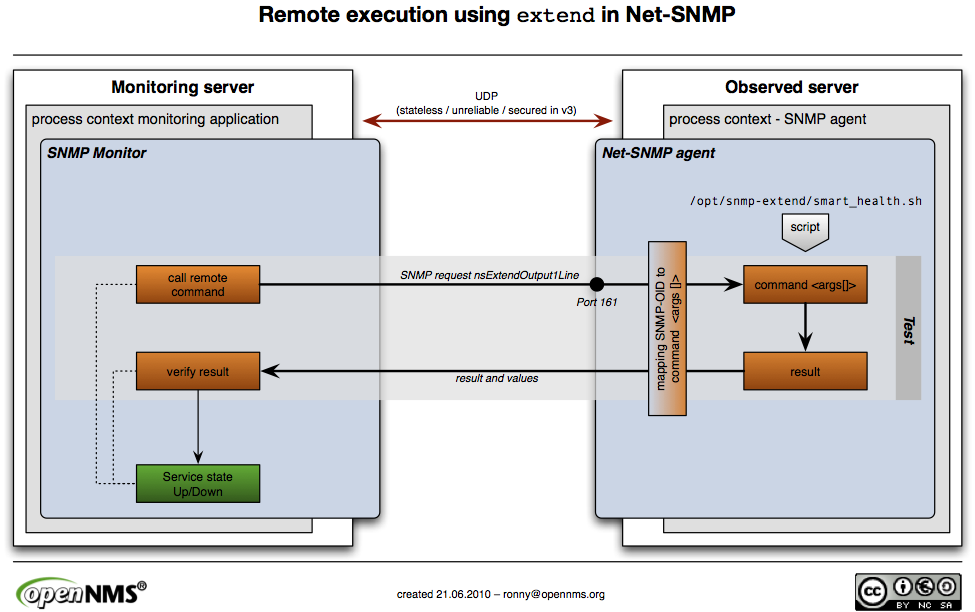
\includegraphics[width=1.0\textwidth]{images/use-cases/script-extending-linux/flow-netsnmp}
	\caption{Ablauf von Abfragen mit der Erweiterung des \emph{Net-SNMP} Agenten}
	\label{pic:flow-netsnmp}
\end{figure}

%=======================================================
\section{Automatisches Service-Recovery}
%=======================================================
Der Einsatz von OpenNMS wird hauptsächlich zu reinen Überwachungszwecken von IT-Systemen verwendet. In manchen Umgebungen kann es hilfreich sein, wenn einfache Wiederherstellungsmassnahemn automatisch ausgeführt werden. Erst wenn diese zu keinem Erfolg führen, wird Benachrichtigung an einen Bereitschaftsmitarbeiter ausgelöst. In diesem Beispiel wird beschrieben wie eine OpenNMS Eskalations-Hierarchie verwendet werden kann um einen solchen Anwendungsfall abzubilden.

WARNUNG: Bei der Umsetzung sollte klar sein, was es bedeutet automatisch ins System einzugreifen und Systemkommandos über entfernte Rechner auszuführen. Zusätzlich sollten Seiteneffekte bezüglich Sicherheit und kennwortloser SSH-authentifizierung berücksichtigt werden. Die Funktionsweise der Eskalation und Benachrichtigung in OpenNMS sollte bekannt sein. Bitte anwenden, wenn Sie wissen was Sie tun.


%=======================================================
\subsection{Beispielszenario mit Web-Servern}
%=======================================================
Im folgenden wird das Konfigurationsszenario kurz beschrieben. In dem gezeigten Beispiel gibt es eine Reihe wichtiger und weniger wichtiger Webserver auf denen Apache2 ausgeführt wird. Die wichtigen Server sind in einer \emph{Surveillance Category} mit der Bezeichnung \emph{VIP-HTTP} zusammenfasst. Für einen Ausfall des Dienstes \emph{HTTP} versucht \emph{OpenNMS} drei mal den \emph{apache2} Dienst neu zu starten bevor eine \emph{SMS\abbrev{SMS}{\markup{S}hort \markup{M}essage \markup{S}ervice}} an den Administrator versendet wird. die folgende Abbildung stellt das Szenario kurz dar.

\begin{figure}[H]
	\centering
	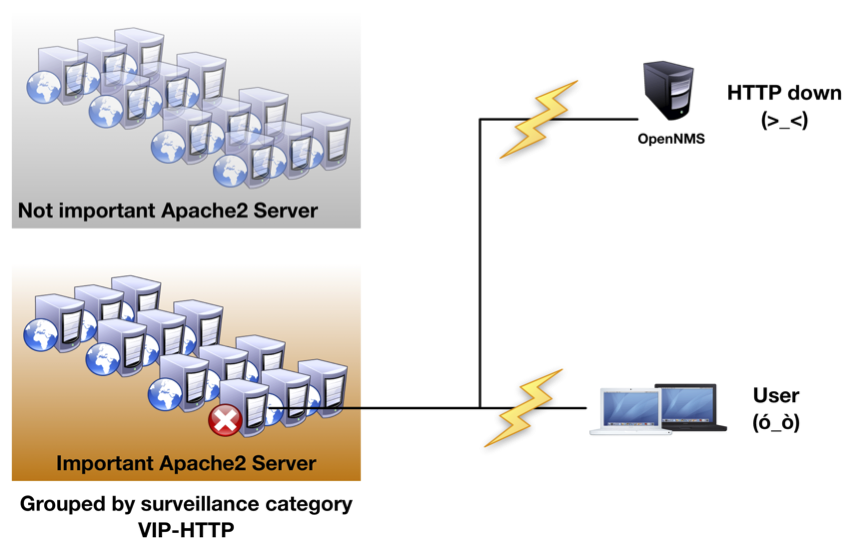
\includegraphics[width=1.0\textwidth]{images/use-cases/service-recovery/szenario}
	\caption{Wiederherstellung am Beispiel von Apache Web-Servern}
	\label{pic:szenario-recovery-apache}
\end{figure}

Für die Einrichtung sind die im folgenden beschriebenen Voraussetzung notwendig. Der Ablauf stellt sich wie folgt dar:

\begin{figure}[H]
	\centering
	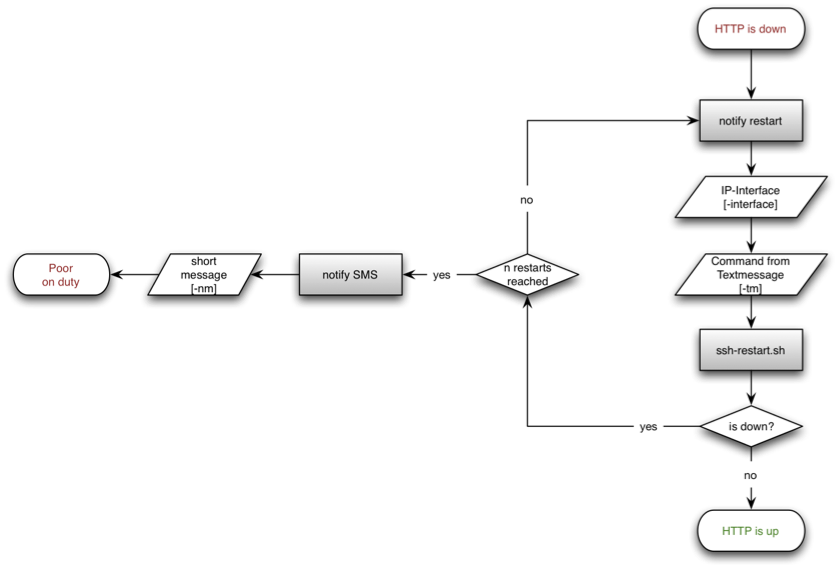
\includegraphics[width=1.0\textwidth]{images/use-cases/service-recovery/notification-workflow}
	\caption{Ablaufdiagram der Benachrichtigung mit Eskalation zur Wiederherstellung des Apache Web-Servers in OpenNMS}
	\label{pic:workflow-recovery-apache}
\end{figure}

%=======================================================
\subsection{Voraussetzungen}
%=======================================================
Der \emph{OpenNMS} Server muss in der Lage sein, entfernte Kommandos per \emph{SSH} ohne Kennworteingabe ausführen können. Dazu kann eine \emph{pubkey-Authentifizierung} eingerichtet werden. Wie \emph{pubkey-Authentifizierung} mit \emph{ssh-keygen} unter Linuxdistributionen eingesetzt wird hier nicht weiter behandelt und auf die Internetseite \url{https://help.ubuntu.com/community/SSH/OpenSSH/Keys} verwiesen. Es ist wichtig, dass \textbf{\textit{KEINE}} \emph{passphrase} verwendet werden darf.

Um einen Serverdienst unter \emph{Linux} neu starten zu können wird übelicherweise eine init-Skript verwendet. In unserem Beispiel wird \emph{Apache2} verwendet. Das init-Skript welches beim Systemstart verwendet wird liegt in 

\begin{lstlisting}[numbers=none]
/etc/init.d/apache2 start|stop|restart
\end{lstlisting}

Der Parameter \emph{restart} kann genutzt werden um einen bereits gestoppten oder fehlerhaft laufenden \emph{apache2} Prozess neu zu starten. Ein \emph{Wrapper-Script} übernimmt diese Aufgabe und kann wie folgt aussehen:

\lstinputlisting[caption={\emph{Wrapper-Skript} um einen service per \emph{SSH} entfernt neu starten zu können}
      \label{lst:ssh-restart-skript}]
  {configs/use-cases/service-recovery/ssh-restart.sh}

Das Skript erwartet drei Parameter und kann wie folgt ausgeführt werden:

\begin{lstlisting}[numbers=none]
ssh-restart.sh <ip-interface> <init-skript> <restart-command>
\end{lstlisting}

Wenn das Kommando vom \emph{OpenNMS} Server auf den zu überwachenden Webserver funktioniert kann mit der Konfiguration der Benachrichtigung in OpenNMS fortgefahren werden.

%=======================================================
\subsection{Benachrichtigung erweitern}
%=======================================================
Das oben gezeigt Skript kann jetzt als neues Kommando für die Benachrichtigung eingerichtet werden. Dazu wird die Datei

\begin{lstlisting}[numbers=none]
$OPENNMS_HOME/etc/notificationCommands.xml
\end{lstlisting}

bearbeitet. \textbf{\textit{Wichtig!}} Es ist darauf zu achten, dass die Pfadangabe in \emph{<execute>...</execute>} korrekt ist.

\lstinputlisting[caption={Benachrichtigung in OpenNMS mit \emph{ssh-restart.sh} erweitern}
      \label{lst:config-notificationCommands}]
  {configs/use-cases/service-recovery/notificationCommands.xml}

Über die \emph{-interface} und \emph{-tm} können über die Benachrichtigung die beiden wichtigen Parameter für unser \emph{SSH-Skript} mit übergeben werden. Nach einem Neustart kann unser \emph{restart-service} im \emph{Destination Path} ausgewählt werden.

%=======================================================
\subsection{Eskalation einrichten}
%=======================================================
Wir erzeugen in der Weboberfläche einen neuen \emph{Destination Path} mit der Bezeichnung \emph{restart-service}. Über die Eskalation wird festgelegt, wie oft versucht werden soll den Dienst neu zu starten. In der folgenden Abbildung ist die Konfiguration dargestellt. Über einen Benutzer \emph{remote} wurde kenntlich gemacht, dass hier ein remote-Kommando drei mal in einem 5-minütigem Abstand ausgeführt werden soll. Falls der \emph{HTTP-Dienst} nach dem dritten mal noch nicht wiederhergestellt ist, wird eine \emph{SMS} an den Benutzer \emph{indigo} gesendet.

\begin{figure}[H]
	\centering
	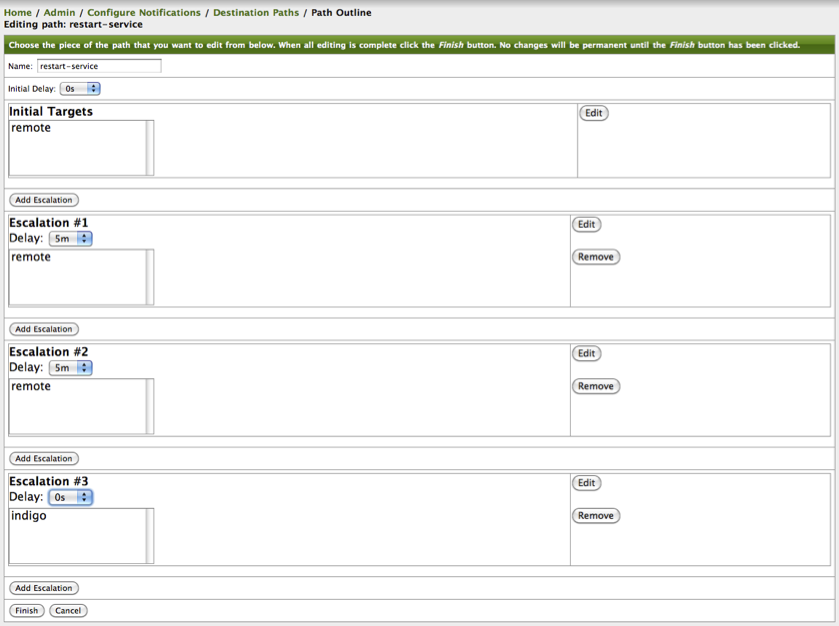
\includegraphics[width=1.0\textwidth]{images/use-cases/service-recovery/escalation}
	\caption{Eskalation für \emph{service-restart} Benachrichtigung}
	\label{pic:escalation-service-restart}
\end{figure}

\textbf{\textit{Wichtig!}} Für den Benutzer \emph{remote} ist zu beachten, dass kein Kommando ausgeführt wird, wenn der Dienst wieder verfügbar ist. Daher hier den Schalter auf \emph{off} setzen. Damit wird verhindert, dass Benachrichtigungen für \emph{RESOLVED-Events} gesendet werden.

\begin{figure}[H]
	\centering
	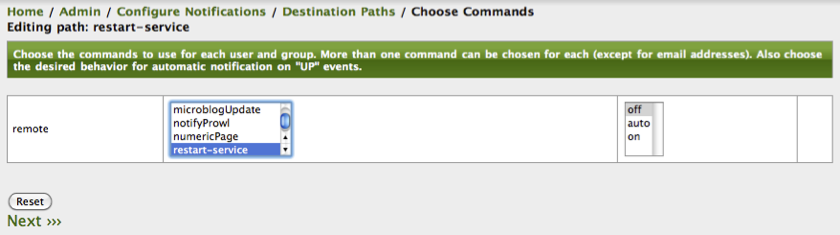
\includegraphics[width=1.0\textwidth]{images/use-cases/service-recovery/destination-path}
	\caption{Konfiguration eines \emph{Destination Path} für \emph{Service-Recovery}}
	\label{pic:destination-path-service-restart}
\end{figure}

Die Benachrichtigung für \emph{SMS} kann wie gewohnt eingerichtet werden. Im nächsten Schritt wird die Konfiguration für das \emph{nodeLostService Event} beschrieben.

\begin{figure}[H]
	\centering
	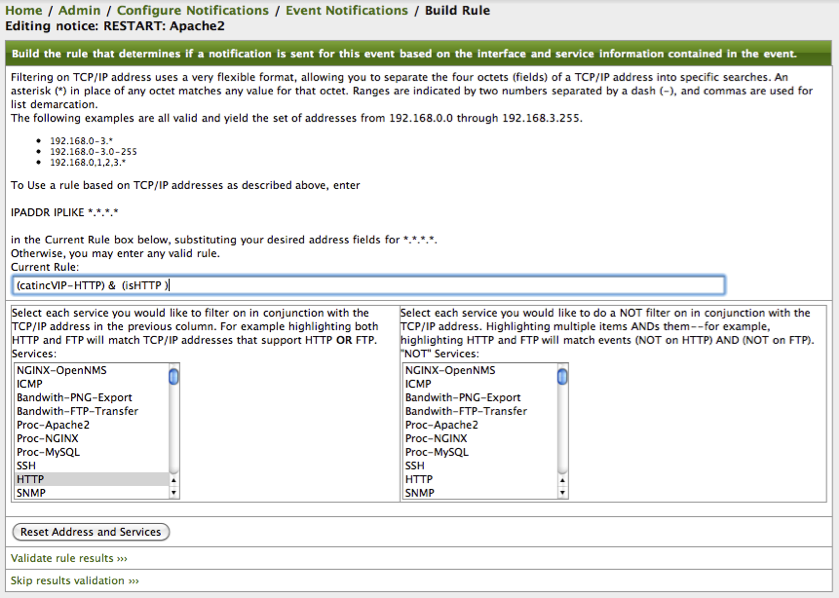
\includegraphics[width=1.0\textwidth]{images/use-cases/service-recovery/notification-rule}
	\caption{Regel für Benachrichtigung für relevante \emph{VIP-HTTP Server}}
	\label{pic:notification-rule-VIP-HTTP}
\end{figure}

Der \emph{Apache2} soll nur für \emph{Nodes} neu gestartet werden die den Service \emph{HTTP} und in der Gruppe \emph{VIP-HTTP} enthalten sind.

\begin{lstlisting}[numbers=none]
(catincVIP-HTTP) & (isHTTP)
\end{lstlisting}

Die Regel kann über \emph{Validate rule } geprüft und dann bestätigt werden. Im nächsten Schritt wird die eigentliche Konfiguration dargestellt. Das Feld \emph{Text Message} hat hier eine besondere Bedeutung. Es enthält den Parameter dem Skript \emph{ssh-restart.sh} mit übergeben wird.

Schlägt das neu starten des \emph{Apache2-Service} fehl, wird eine \emph{SMS} versendet. Diese Benachrichtigung verwendet das \emph{Short Message} Textfeld als Nachrichtentext.

\begin{figure}[H]
	\centering
	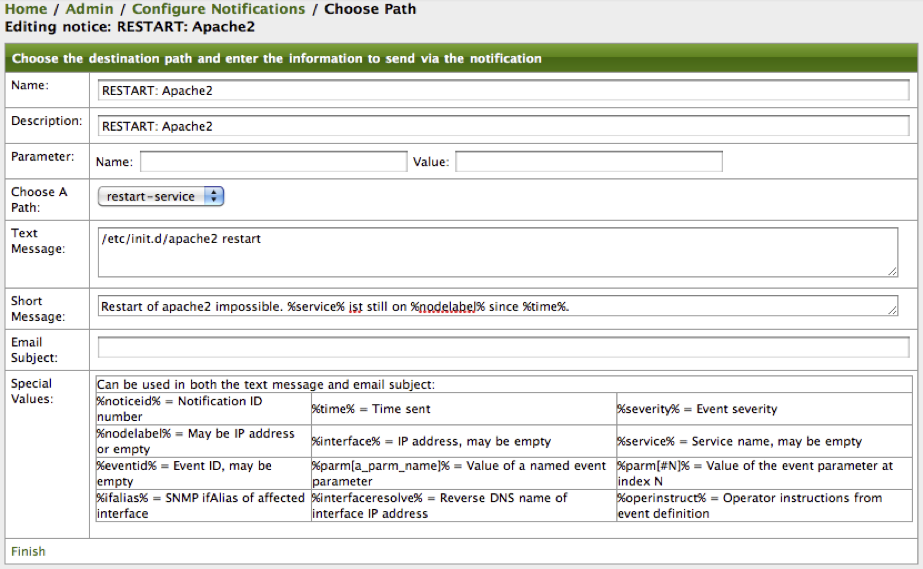
\includegraphics[width=1.0\textwidth]{images/use-cases/service-recovery/notification-text}
	\caption{Text für die Benachrichtigung und \emph{restart service} Kommando.}
	\label{pic:notification-text}
\end{figure}

Es wird das Kommando \emph{/etc/init.d/apache2 restart} an das \emph{notification command} übergeben. Mit dem angelegten \emph{Destination path} können beliebige Dienste neu gestartet werden. Die Meldung in \emph{Short Message} wird nach dem dritten Versuch des Neustarts als \emph{SMS-Text} versendet.

\include{content/use-cases/service-assurance/http-monitor}

\lstlistoflistings
\addcontentsline{toc}{chapter}{Listings}

\end{document}
